% Paquets généraux
\documentclass[a4paper,12pt,titlepage,twoside]{article}
\usepackage[T1]{fontenc}
\usepackage[utf8]{inputenc}
\usepackage[french]{babel}
\addto\captionsfrench{%
  \renewcommand{\tablename}{Tableau}%
}
\usepackage[gen]{eurosym}
%\usepackage[dvips]{graphicx}
\usepackage{fancyhdr}
\usepackage{pdfpages} 
\usepackage{multido}
\usepackage{hyperref}
%\usepackage{textcomp}
\usepackage{schemabloc}
\usepackage[bitstream-charter]{mathdesign}
\usepackage{array}
\newcolumntype{P}[1]{>{\centering\arraybackslash}p{#1}}

\newcommand{\id}{54}
\newcommand{\nom}{Liaisons mécaniques}
\newcommand{\sequence}{04}
\newcommand{\num}{01}
\newcommand{\type}{TP}
\newcommand{\descrip}{Modélisation d'un solide. Comportement des liaisons mécaniques. Modéliser les mécanismes du laboratoire par un schéma cinématique, paramétré.}
\newcommand{\competences}{A3-C4: Analyse d'architecture et de comportement \\ &  Mod1-C1: Isolement d'un solide ou d'un système de solides \\ &  Mod2-C10-1: Modèle de solide indéformable \\ &  Mod2-C11: Modélisation géométrique et cinématique des mouvements entre solides indéformables \\ &  Mod2-C12: Modélisation cinématique des liaisons entre solides \\ &  Mod2-C15: Modélisation des actions mécaniques \\ &  Rés-C6: Utilisation d'un solveur ou d'un logiciel multi physique \\ &  Com1-C1: Différents descripteurs introduits dans le programme \\ &  Com2-C4: Outils de communication}
\newcommand{\nbcomp}{9}
\newcommand{\systemes}{Plateforme Stewart}
\newcommand{\systemessansaccent}{Plateforme Stewart}
\newcommand{\ilot}{2}
\newcommand{\ilotstr}{02}
\newcommand{\dossierilot}{\detokenize{Ilot_02 Plateforme Stewart}}
\newcommand{\imageun}{Plateforme}

\newcommand{\urlsysteme}{\href{https://www.costadoat.fr/systeme/57}{Ressources système}}
\newcommand{\matlabsimscape}{\href{https://github.com/Costadoat/Sciences-Ingenieur/raw/master/Systemes/Plateforme Stewart/Plateforme_Stewart_Simscape.zip}{Modèle Simscape}}
\newcommand{\solidworks}{\href{https://github.com/Costadoat/Sciences-Ingenieur/raw/master/Systemes/Plateforme Stewart/Plateforme_Stewart_Solidworks.zip}{Modèle Solidworks}}
\newcommand{\edrawings}{\href{https://github.com/Costadoat/Sciences-Ingenieur/raw/master/Systemes/Plateforme Stewart/Plateforme_Stewart.EASM}{Modèle eDrawings}}
\newcommand{\test}{Stewart_param1}
\newcommand{\testi}{Stewart_param2}
\newcommand{\testii}{Stewart_param3}
\newcommand{\testiii}{Stewart_param4}
\newcommand{\testiiii}{Stewart_euler}

\newcommand{\institute}{Lycée Dorian}

\usepackage{fancyvrb}
\usepackage{color}
\usepackage{xcolor}
\usepackage{colortbl}
\usepackage{helvet}
\renewcommand{\familydefault}{\sfdefault}
\usepackage{amsfonts}
\usepackage{amsmath}
%\usepackage{xspace}
\usepackage{varioref}
\usepackage{tabularx}
%\usepackage{floatflt}
\usepackage{graphics}
\usepackage{wrapfig}
\usepackage{textcomp}
\usepackage{tikz}
\usepackage{wrapfig}
\usepackage{gensymb}
\usepackage[percent]{overpic}
\usepackage[european]{circuitikz}
\usetikzlibrary{babel}
\usepackage{ifthen}
\usepackage{cancel}
\usepackage{etoolbox}
\usepackage{multirow}
%\usepackage{boxedminipage}
\definecolor{gris25}{gray}{0.75}
\definecolor{bleu}{RGB}{18,33,98}
\definecolor{bleuf}{RGB}{42,94,171}
\definecolor{bleuc}{RGB}{231,239,247}
\definecolor{rougef}{RGB}{185,18,27}
\definecolor{rougec}{RGB}{255,188,204}%255,230,231
\definecolor{vertf}{RGB}{103,126,82}
\definecolor{vertc}{RGB}{220,255,191}
\definecolor{forestgreen}{rgb}{0.13,0.54,0.13}
\definecolor{blcr}{rgb}{0.59,0.69,0.84}
\definecolor{blfr}{rgb}{0.32,0.51,0.75}
\definecolor{orfr}{rgb}{0.90,0.42,0.15}
\definecolor{orcr}{rgb}{0.90,0.65,0.50}
\definecolor{orangef}{rgb}{0.659,0.269,0.072}
\definecolor{orange}{rgb}{0.58,0.35,0.063}
\definecolor{orangec}{rgb}{0.43,0.32,0.25}
\definecolor{rcorrect}{rgb}{0.6,0,0}
\definecolor{sequence}{rgb}{0.75,0.75,0.75}
\definecolor{competences}{rgb}{0.61,0.73,0.35}
\definecolor{grisf}{HTML}{222222}
\definecolor{grisc}{HTML}{636363}
\definecolor{normal}{HTML}{4087c4}
\definecolor{info}{HTML}{5bc0de}
\definecolor{success}{RGB}{92,184,92}
\definecolor{warning}{RGB}{240,173,78}
\definecolor{danger}{RGB}{217,83,79}
\hypersetup{                    % parametrage des hyperliens
    colorlinks=true,                % colorise les liens
    breaklinks=true,                % permet les retours à la ligne pour les liens trop longs
    urlcolor= blfr,                 % couleur des hyperliens
    linkcolor= orange,                % couleur des liens internes aux documents (index, figures, tableaux, equations,...)
    citecolor= forestgreen                % couleur des liens vers les references bibliographiques
    }

% Mise en page
\pagestyle{fancy}

\setlength{\hoffset}{-18pt}
\setlength{\oddsidemargin}{0pt} 	% Marge gauche sur pages impaire2s
\setlength{\evensidemargin}{0pt} 	% Marge gauche sur pages paires
\setlength{\marginparwidth}{00pt} 	% Largeur de note dans la marge
\setlength{\headwidth}{481pt} 	 	% Largeur de la zone de tête (17cm)
\setlength{\textwidth}{481pt} 	 	% Largeu\textbf{r de la zone de texte (17cm)
\setlength{\voffset}{-18pt} 		% Bon pour DOS
\setlength{\marginparsep}{7pt}	 	% Séparation de la marge
\setlength{\topmargin}{-30pt} 		% Pas de marge en haut
\setlength{\headheight}{55pt} 		% Haut de page
\setlength{\headsep}{20pt} 		% Entre le haut de page et le texte
\setlength{\footskip}{30pt} 		% Bas de\textbf{ page + séparation
\setlength{\textheight}{700pt} 		% Hauteur de l'icone zone de texte (25cm)
\setlength\fboxrule{1 pt}
\renewcommand{\baselinestretch}{1}
\setcounter{tocdepth}{1}
\newcommand{\cadre}[2]
{\fbox{
  \begin{minipage}{#1\linewidth}
   \begin{center}
    #2\\
   \end{center}
  \end{minipage}
 }
}

\newcommand{\repon}[1]
{
~\ \\
\begin{tabular}{|m{\linewidth}|}
 \hline
\multido{}{#1}{\\ \hline}
\end{tabular}
}

\newcounter{num_quest} \setcounter{num_quest}{0}
\newcounter{num_rep} \setcounter{num_rep}{0}
\newcounter{num_cor} \setcounter{num_cor}{0}

\newcommand{\question}[1]{\refstepcounter{num_quest}\par
~\ \\ \parbox[t][][t]{0.15\linewidth}{\textbf{Question \arabic{num_quest}}}\parbox[t][][t]{0.85\linewidth}{#1}\par
}


\newcommand{\reponse}[3]
{\refstepcounter{num_rep}
\noindent
\rule{\linewidth}{.5pt}\\
\textbf{Question \arabic{num_rep}:} ~\ \\
\ifdef{\public}{\multido{\i=1+1}{#1}{~\ \\}#2}{#3}
}

\newcommand{\cor}
{\refstepcounter{num_cor}
\noindent
\rule{\linewidth}{.5pt}
\textbf{Question \arabic{num_cor}:} \\
}

\newcommand{\repcarre}[2]
{
~\ \\
\begin{tikzpicture}
\draw [fill=white] (0,0) rectangle +(\linewidth,#1);
\node[align=left] at (1.1,#2-0.3) {\textbf{Question #1:}};
\end{tikzpicture}
}

\newcommand{\titre}[1]
{\begin{center}
\cadre{0.8}{\huge #1} 
\end{center}
}


% En tête et pied de page
\lhead{\nom}
\rhead{
\includegraphics[width=2cm]{../../img/logo}}
\lfoot{\auteurun,\ \auteurdeux}
\cfoot{Page \thepage}

\fancypagestyle{documentreponse}{%
  \fancyhf{}
  \fancyhead[LO]{Nom: ........................ Prénom: ........................}
  \fancyhead[LE]{\nom}
  \fancyhead[RE,RO]{
\includegraphics[width=2cm]{../../img/logo}}
  \lfoot{Document réponse}
  \cfoot{Page \thepage}
   }
  
\fancypagestyle{correction}{%
  \fancyhf{}
  \lhead{\colorbox{danger}{\begin{minipage}{0.65\paperwidth} \textcolor{white}{\textbf{Correction}} \end{minipage}} }
  \rhead{
\includegraphics[width=2cm]{../../img/logo}}
  \lfoot{Renaud Costadoat, Françoise Puig}
  \rfoot{\colorbox{danger}{\begin{minipage}{0.5\paperwidth} \begin{flushright}\textcolor{white}{\textbf{Correction}}\end{flushright} \end{minipage}} }}

\fancypagestyle{correctioninfo}{%
  \fancyhf{}
  \lhead{\colorbox{danger}{\begin{minipage}{0.65\paperwidth} \textcolor{white}{\textbf{Correction}} \end{minipage}} }
  \rhead{
\includegraphics[width=2cm]{../../img/logo}}
  \lfoot{Renaud Costadoat, Juliette Genzmer, Willie Robert}
  \rfoot{\colorbox{danger}{\begin{minipage}{0.6\paperwidth} \begin{flushright}\textcolor{white}{\textbf{Correction}}\end{flushright} \end{minipage}} }}

\renewcommand{\footrulewidth}{0.4pt}

\usepackage{eso-pic}
\newcommand{\BackgroundPic}{%
\put(0,0){%
\parbox[b][\paperheight]{\paperwidth}{%
\vfill
\begin{center}
\hspace{0.5cm}\vspace{0.5cm}

\includegraphics[width=\paperwidth,height=\paperheight,%
keepaspectratio]{../../img/fond3}%
\end{center}
\vfill
}}}

\newcommand{\BackgroundPicdeux}{%
\put(25,-30){%
\parbox[b][\paperheight]{\paperwidth}{%
\vfill
\begin{center}
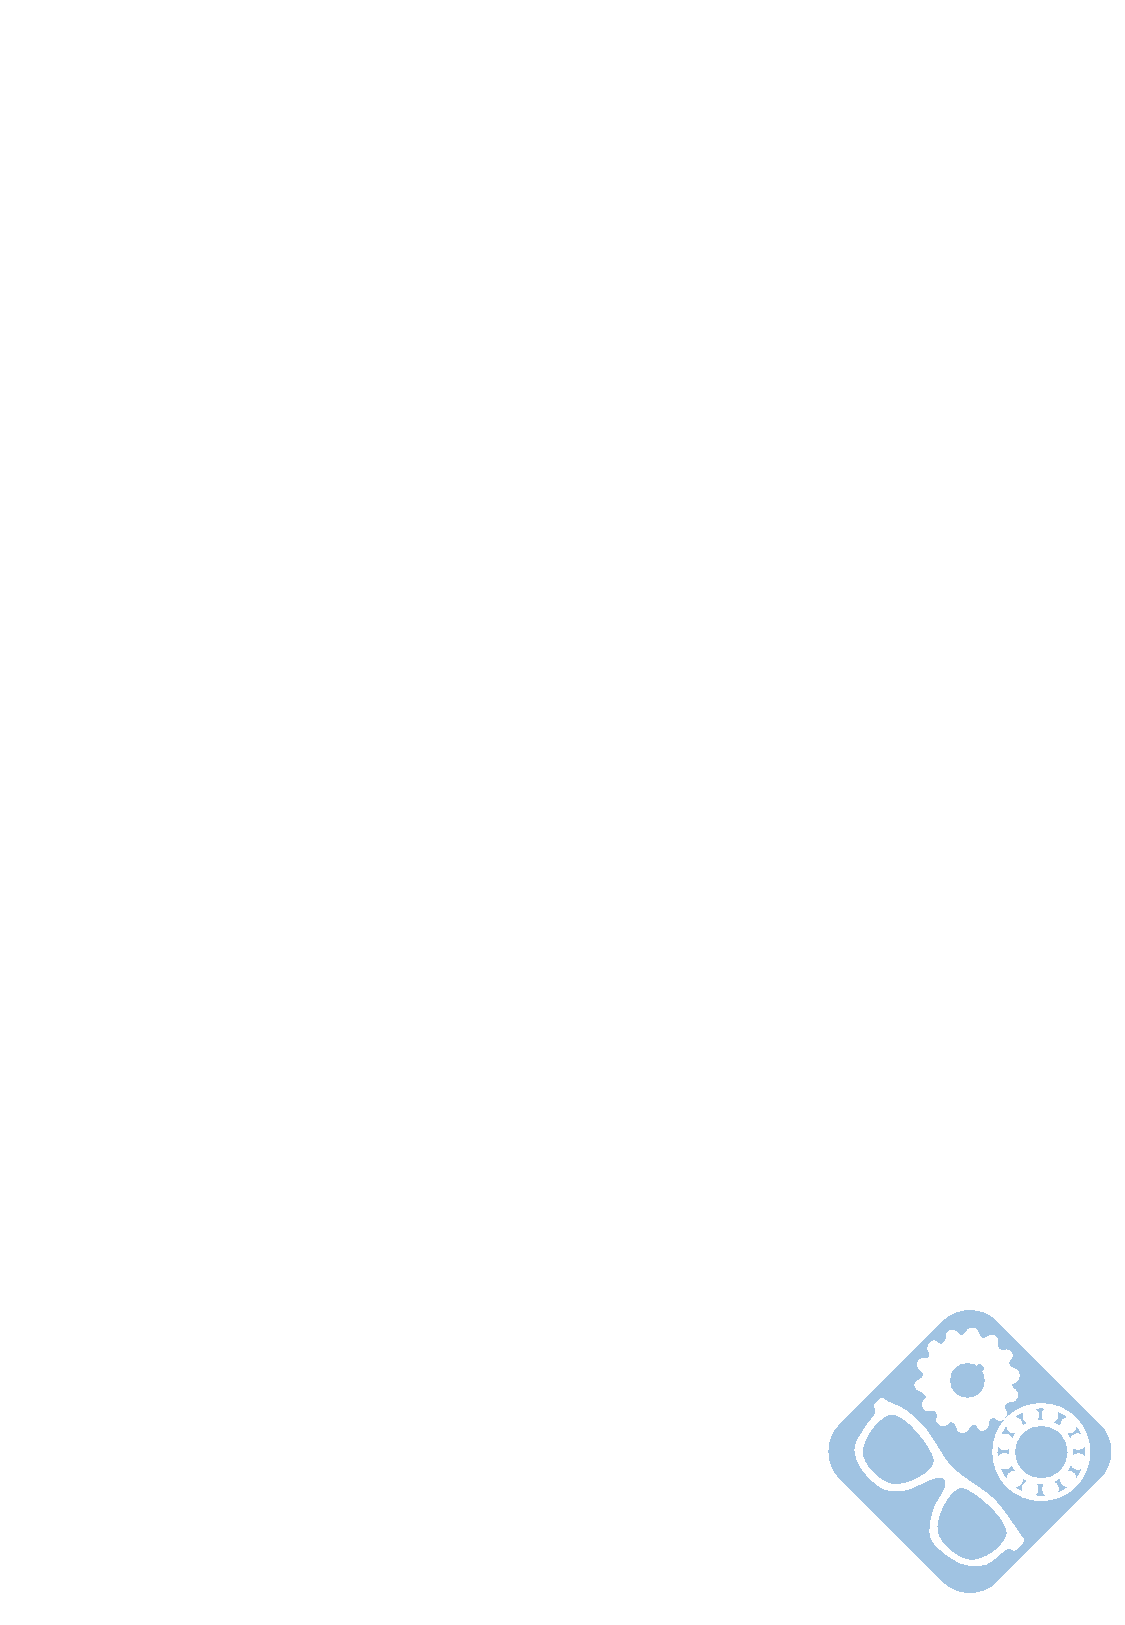
\includegraphics[width=\paperwidth,height=\paperheight,%
keepaspectratio]{../../img/fond4}%
\end{center}
\vfill
}}}

\begin{document}

\pagestyle{empty}

\AddToShipoutPicture*{\BackgroundPic}


\includegraphics[width=2cm]{../../img/logo}

\Huge{DS \num\ - \sujet}

\vspace{1cm}

\ifdef{\prive}{\begin{center}\colorbox{danger}{\Huge{Avec Correction}}\end{center}}{}

\begin{center}
\centering\huge{PTSI}
\end{center}

\vspace{2cm}


\begin{center}
\centering\Large{\jour}
\end{center}

\vspace{2cm}

\normalsize

\tableofcontents

\newpage

\AddToShipoutPicture{\BackgroundPicdeux}

\pagestyle{fancy}

\begin{center}
\Huge \sujet
\end{center}


\normalsize

\textbf{Les copies sont en séparer en trois parties:
\begin{enumerate}
 \item  Questions 1 à 20,
 \item Questions 21 à 34,
 \item Document réponse.
\end{enumerate}}

\section{Découverte du système}

Le panneau publicitaire déroulant, appartenant à la catégorie des MUPI (Mobilier Urbain Pour l'Information), est un objet installé dans l'espace public. C'est un media de masse qui permet de toucher le consommateur sur son lieu de vie. La société JC DECAUX qui installe des mobiliers urbains fixes s'est intéressée depuis longtemps à pouvoir toucher un maximum de personnes grâce à l'utilisation de ces panneaux.

\begin{wrapfigure}{r}{50mm}
  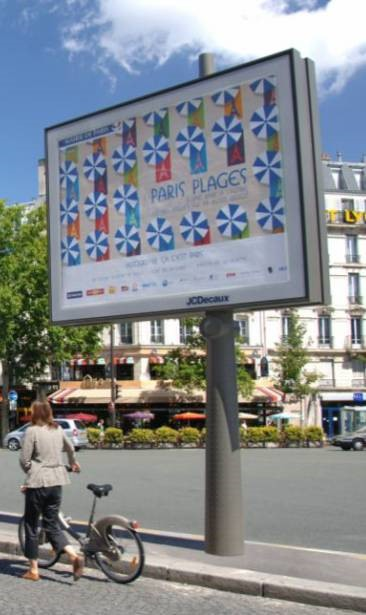
\includegraphics[width=0.9\linewidth]{img/fig00a}
  \label{fig00a}
  \caption{Panneau déroulant}
\end{wrapfigure}

En effet, on a longtemps utilisé des panneaux fixes mais les études réalisées par JC Decaux Wordlink ont permis d'analyser les effets publicitaires de l'introduction du mouvement dans la communication extérieure.
Cette étude, appelée Sutton démontre qu'un panneau en mouvement augmente le contact visuel avec le panneau de 37\%. Ceci signifie que 90\% du trafic aura au moins un contact visuel avec le site durant son passage. Lorsque le panneau est déroulant, plus de deux-tiers de personnes mémorisent la campagne. C'est pourquoi JC DECAUX a été amené à développer ce type de panneau déroulant. L'expérience de JC DECAUX dans ce domaine date de plus de trente ans puisque le premier brevet concernant ce type de panneau a été déposé en décembre 1977.

Le système étudié est le système de panneau type sénior de $8m^2$ qui équipe de nombreuses villes dont Paris.
Ce panneau permet de faire défiler successivement dans un sens puis dans l'autre jusqu'à 7 affiches avec un temps d'exposition constant pour chaque affiche. 

Le système actuel est décrit en annexe 1.

\subsection{Mise en situation}

Le format des affiches rétro éclairées est d'environ $8m^2$.

\begin{figure}[!h]
\begin{center}
	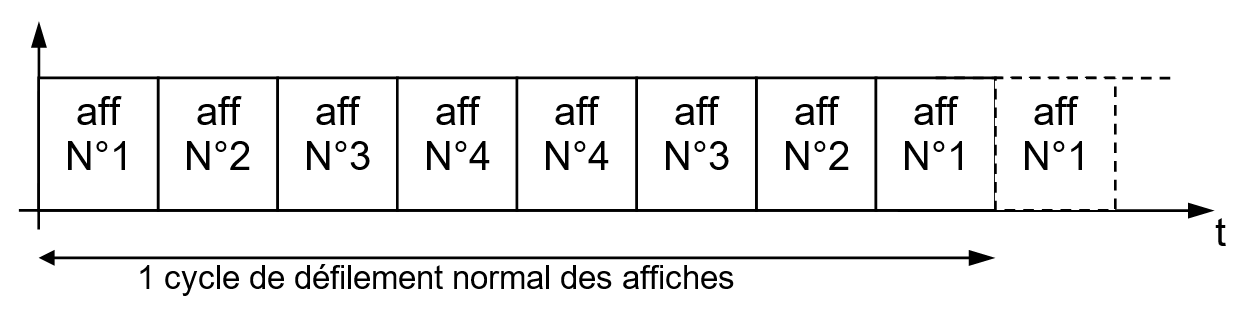
\includegraphics[width=0.6\linewidth]{img/fig00b}
\end{center}
	\label{fig00b}
	\caption{Défilement pour 4 affiches}
\end{figure}

Les affiches sont de dimensions : 3200 x 2300 mm (largeur x hauteur) avec une surface visible de 3060 x 2230 mm.

Le défilement s'effectue à la vitesse de 1m/s avec une rampe d'accélération et de décélération de chacune 1 seconde.

\begin{wrapfigure}{r}{50mm}
  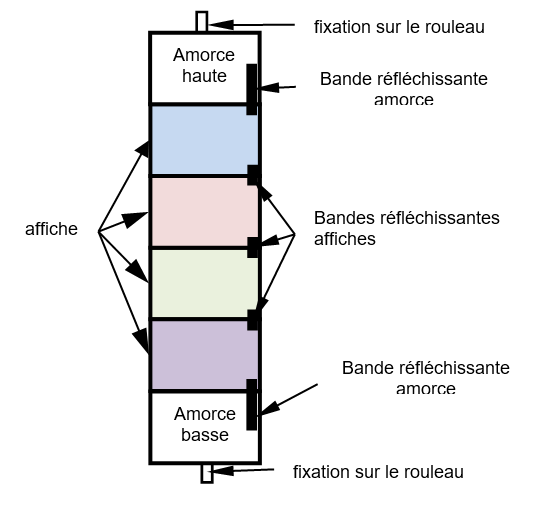
\includegraphics[width=0.9\linewidth]{img/fig00c}
  \label{fig00c}
  \caption{Affiches}
\end{wrapfigure}

Les affiches étant changées tous les 15 jours,  il faut faciliter leur mise en place. Pour cela, elles sont disposées en bandeau et placées sur le rouleau du haut lors de leur installation. La première est une amorce fixée au rouleau du haut avec un adhésif puis elles sont reliées les unes aux autres par un système de zip. La dernière est une amorce qui est également fixée au rouleau du bas par un adhésif. Cet ensemble constitue un bandeau.

Dans la solution actuelle, l'entraînement se fait par deux moteurs asynchrones identiques commandés par deux variateurs scalaires. L'ensemble est géré par l'automate programmable.

\subsection{Diagramme des cas d'utilisation}

\begin{figure}[!h]
\begin{center}
	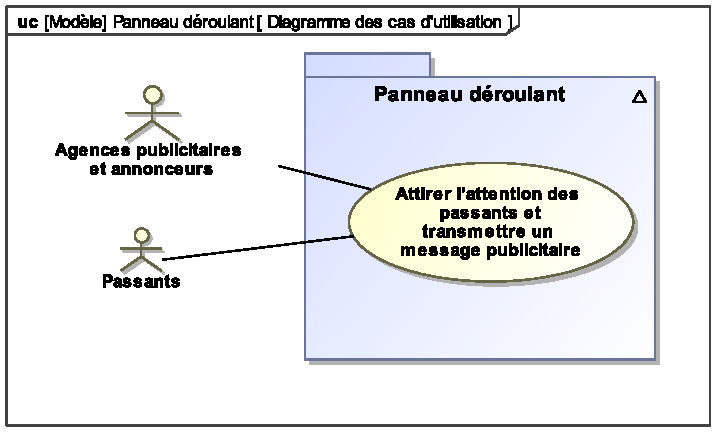
\includegraphics[width=0.5\linewidth]{img/use_case}
\end{center}
	\label{use_case}
	\caption{Diagramme des cas d'utilisation}
\end{figure}

\subsection{Diagramme de contexte}

\begin{figure}[!h]
\begin{center}
	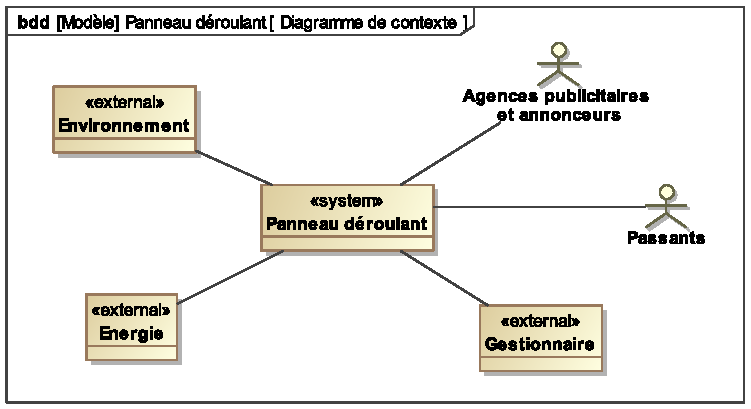
\includegraphics[width=0.5\linewidth]{img/contexte}
\end{center}
	\label{contexte}
	\caption{Diagramme de contexte}
\end{figure}

~\

\subsection{Diagramme d'exigences}

~\

\begin{figure}[!h]
\begin{center}
	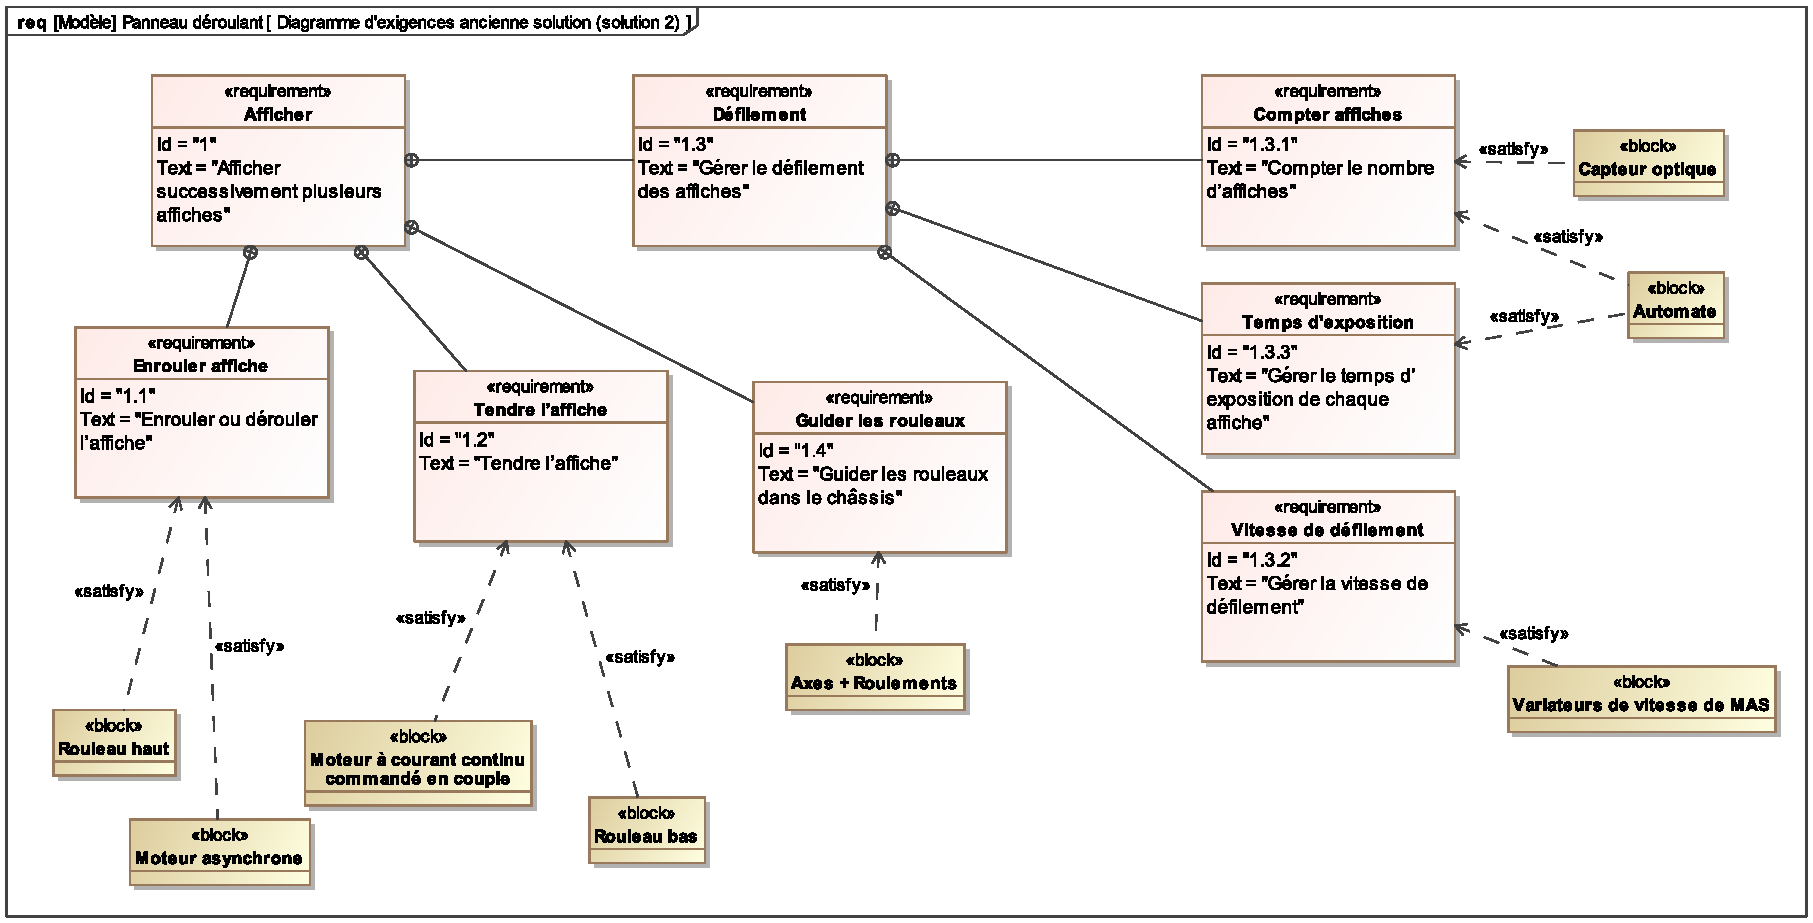
\includegraphics[width=0.9\linewidth]{img/exigences_sol2}
\end{center}
	\label{use_case}
	\caption{Diagramme d'exigence de l'ancienne solution (solution 2)}
\end{figure}

\begin{figure}[!h]
\begin{center}
	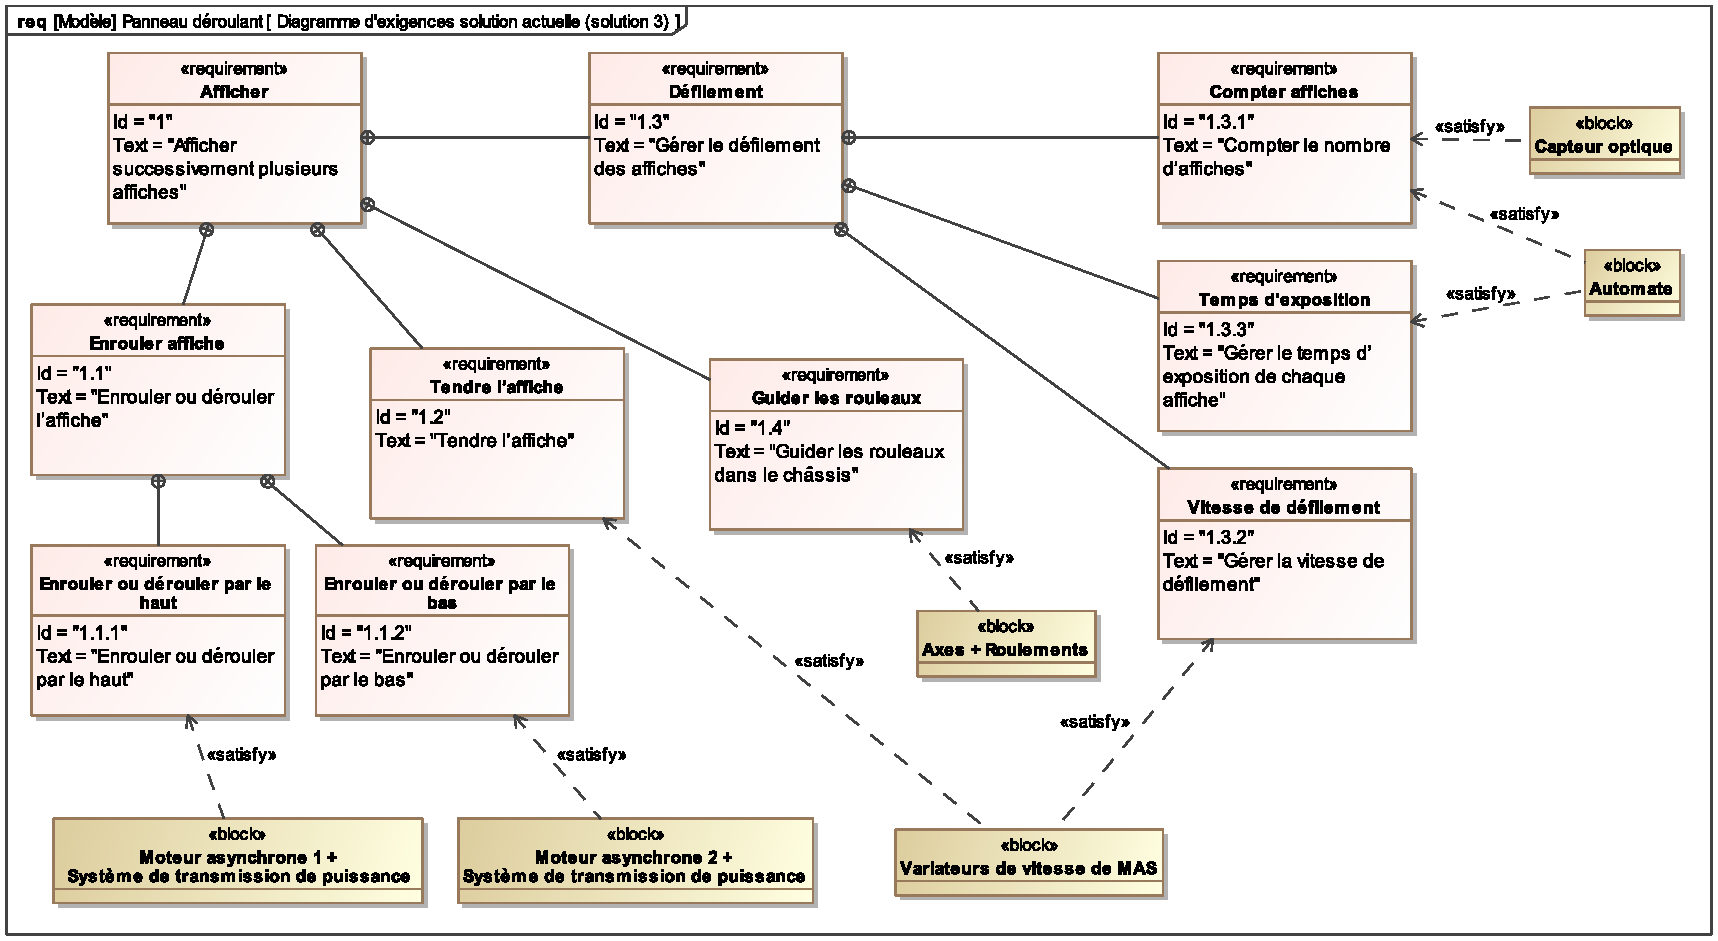
\includegraphics[width=0.9\linewidth]{img/exigences_sol3}
\end{center}
	\label{use_case}
	\caption{Diagramme d'exigence de la solution actuelle (solution 3)}
\end{figure}

~\

\section{Étude de la fonction : « enrouler ou dérouler l'affiche »}

On s'intéresse ici au rouleau supérieur du panneau d'affichage et on considère que le bandeau d'affiches s'enroule sur ce rouleau supérieur.

L'étude du comportement dynamique du système nous amène à chercher la masse du rouleau.

Hypothèses :
\begin{itemize}
 \item le rouleau supérieur vide est un cylindre creux en aluminium de longueur L, de diamètre intérieur $d_1$  et de diamètre extérieur $d_2$,
 \item une fois entièrement enroulé autour du rouleau supérieur, le bandeau d'affiches est un cylindre creux de longueur L=3200 mm, de diamètre intérieur $d_2$ et de diamètre extérieur $d_3$.
\end{itemize}
 
\begin{figure}[!h]
\begin{center}
	
\includegraphics[width=\linewidth]{img/fig01}
\end{center}
	\caption{Modèle pour le calcul de la masse}
	\label{fig01}
\end{figure}

On donne: $0,14^2=0,0196$, $0,129^2=0,0166$ et $0,152^2=0,0231$.

\question{Donner l'expression de la masse du rouleau $M_{roul}$ en fonction de $\rho_{roul}$, L, $d_1$ et $d_2$.
Calculer $M_{roul}$.}

\question{Donner l'expression de la masse du bandeau d'affiches $M_{b}$ en fonction de $\rho_{b}$, L, $d_2$ et $d_3$. Calculer $M_{b}$.}

~\

La figure \ref{fig02} présente un modèle du montage des roulements qui supportent les rouleaux.

\begin{figure}[!h]
	\centering 
	\begin{overpic}[width=0.6\textwidth]{img/fig02}
 \put (10,22) {A}
 \put (98,22) {B}
 \put (52,20) {G}
 \put (52,0) {$\overrightarrow{P_{roul}}+\overrightarrow{P_b}$}
\end{overpic}
	\caption{Montage rouleau}
	\label{fig02}
\end{figure}

\question{Déterminer les actions dans les liaisons en A et en B.}

\question{En déduire les actions radiales que supportent ces roulements.}

\subsection{Détermination de la loi de variation de la vitesse angulaire du rouleau au cours de l'enroulement des affiches}

Lors de l'enroulement sur le rouleau, on souhaite respecter la loi cinématique suivante :
 
\begin{figure}[!h]
\begin{center}
	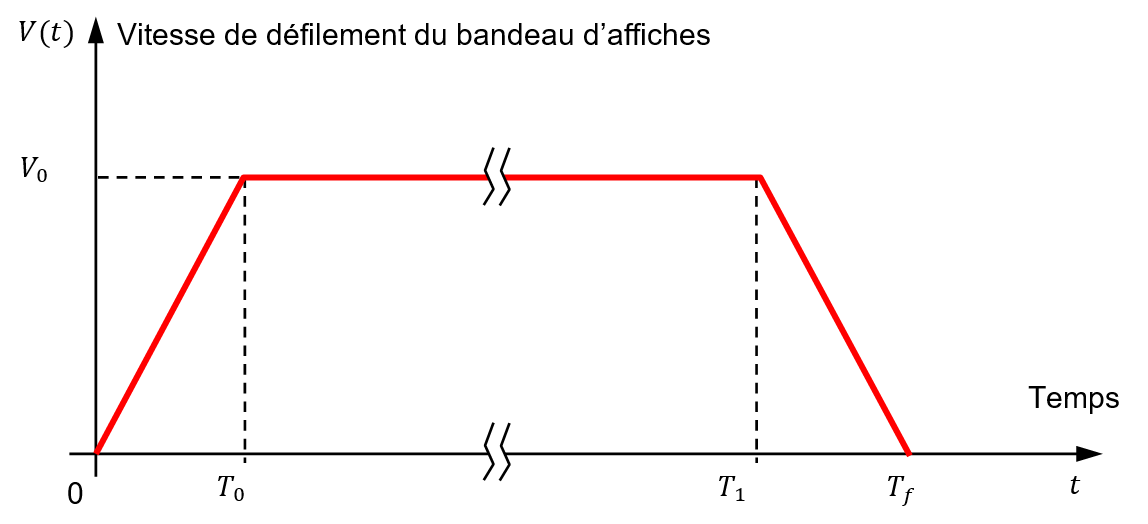
\includegraphics[width=0.5\linewidth]{img/fig03}
\end{center}
	\caption{Loi cinématique de défilement d'une affiche du bandeau}
	\label{fig03}
\end{figure}

On s'intéresse à la phase durant laquelle $V(t)=V_0=$constante.

On utilise le modèle suivant pour l'étude de l'enroulement des affiches :
  
\begin{figure}[!h]
\begin{center}
	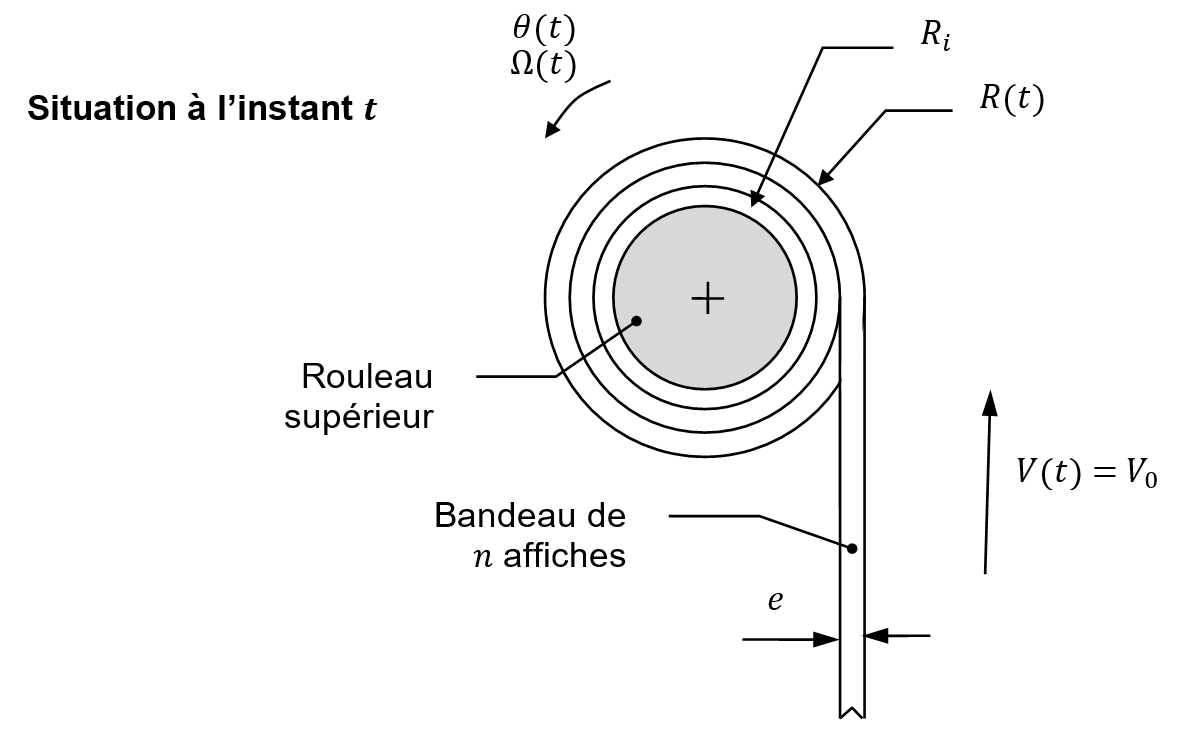
\includegraphics[width=0.5\linewidth]{img/fig04}
\end{center}
	\caption{Modèle pour l'enroulement des affiches sur le rouleau supérieur}
	\label{fig04}
\end{figure}

\newpage

\textbf{Données complémentaires :}
\begin{itemize}
 \item Rouleau :
\begin{itemize}
 \item Rayon initial : $\frac{d_2}{2}=R_i=70 mm$,
 \item Rayon en cours d'enroulement : $R(t)$,
 \item Rayon final : $\frac{d_3}{2}=R_f$,
 \item Position angulaire du rouleau par rapport au bâti : $\theta(t)$,
 \item Vitesse angulaire du rouleau par rapport au bâti : $\Omega(t)$.
\end{itemize} 
 \item Affiche :
\begin{itemize}
 \item Hauteur d'une affiche : $H=2300 mm$,
 \item Largeur d'une affiche : $L=3200 mm$,
 \item Épaisseur d'une affiche : $e=200 \mu m$,
 \item Vitesse de défilement en régime établi : $V_0=1 m.s^{-1}$,
\end{itemize}
 \item Bandeau :
\begin{itemize}
 \item Nombre d'affiches sur le bandeau : $n=6$,
 \item Longueur du bandeau (affiches + amorces) : $L_b=15m$. 
\end{itemize}
\end{itemize}

~\

On adopte la loi de variation suivante pour $R(t)$:\\
\begin{center}
$R(t)=R_i+\left[\frac{\theta(t)}{2\cdot\pi}\right]\cdot e$
\end{center}

La vitesse d'enroulement V(t) est maintenue constante :\\
\begin{center}
$V_0=R(t)\cdot\Omega(t)=$constante avec $\Omega(t)=\frac{d\theta(t)}{dt}$
\end{center}

~\

\question{Par dérivation de l'expression de $R(t)$ par rapport au temps, montrer que l'on peut écrire :}

\begin{center}
$\frac{dR(t)}{dt}=\left[\frac{e}{2.\pi}\right].\frac{V_0}{R(t)}$
\end{center}

\question{En utilisant la condition initiale $R(0)=R_i$, montrer que l'expression suivante \\
$R(t)=\sqrt{R_i^2+\frac{e}{\pi}\cdot V_0\cdot t}$ est solution de l'équation précédente.}

\question{En négligeant la durée des phases d'accélération et de décélération de la loi cinématique de la figure \ref{fig03} vis-à-vis de la durée de la phase à vitesse constante, calculer la valeur du rayon final $R_f$ si on considère que $T_f=14 s$.}

\question{Exprimer puis calculer les vitesses angulaires maximale $\Omega_{max}$ et minimale $\Omega_{min}$ du rouleau au cours de l'enroulement.}

\question{Calculer l'écart relatif $\frac{\Omega_{max}-\Omega_{min}}{\Omega_{max}}$ et conclure sur l'évolution de la vitesse angulaire du rouleau au cours de l'enroulement (ou du déroulement) de l'affiche.}

~\

Dans toute la suite du sujet, on considèrera qu'en maintenant la vitesse angulaire des rouleaux constante pendant les phases d'enroulement et de déroulement du bandeau d'affiches, on respecte le cahier des charges fonctionnel.

Le rayon $R(t)$ pourra donc être considéré comme constant pendant l'enroulement du bandeau. Il sera noté $R$ avec $R=76 mm$.

\section{Étude de la fonction : « gérer le défilement des affiches »}

La gestion du défilement des affiches s'effectue par un automate programmable de type Siemens S7-216. 

\begin{wrapfigure}{r}{70mm}
  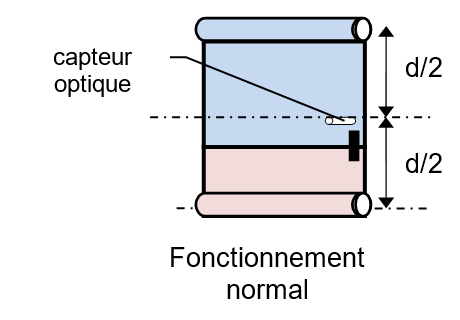
\includegraphics[width=0.9\linewidth]{img/fig06}
  \caption{Bandeau d'affiches sur les rouleaux (vue arrière)}
  \label{fig06}
\end{wrapfigure}

Le système dispose d'un capteur optique situé sur le coté arrière à égale distance des deux rouleaux. La distance 
\og d \fg entre les deux rouleaux est de 2300 mm.

Les affiches (3200 x 2300 mm) sont reliées entre elles par un procédé ZipGrip et renforcées par une bande adhésive. Sur le bord de celles-ci est placée une bande réfléchissante de 50 x 150 mm à cheval sur les deux affiches. Aux extrémités des affiches se trouvent des amorces (support d'affiche de même longueur) avec des bandes réfléchissantes 50 x 600 mm.

Lors d'un défilement normal, le capteur ne voit que les bandes réfléchissantes d'affiche (brAf).

~\ \\ ~\

\textbf{Hypothèses :}\\

Pour simplifier l'étude, on supposera qu'un seul moteur (moteur haut ou bas) est commandé à la fois pour enrouler l'affiche sur son rouleau.

Les commandes MH et MB pilotent les mises en marche et l'arrêt des variateurs associés aux moteurs, c'est-à-dire qu'elles déclenchent les rampes d'accélération et décélération des moteurs.

On s'intéresse à deux aspects du défilement des affiches que sont la commande du moteur d'entraînement et la mise en forme du signal provenant du capteur optique.

\subsection{Réglage de la temporisation de commande du moteur d'entraînement}

Le but est de déterminer les paramètres de réglage de l'automate pour obtenir le positionnement correct des affiches.

Lors du défilement des affiches, on constate que l'arrêt ne doit pas s'effectuer lors du passage de la bande réfléchissante d'affiche mais après un temps $T_p$ qui doit être programmé dans l'automate.

Lors du fonctionnement normal, la commande des moteurs s'effectue suivant le cycle dans lequel $T_{exp}$ représente le temps d'exposition :
 
\begin{figure}[!h]
\begin{center}
	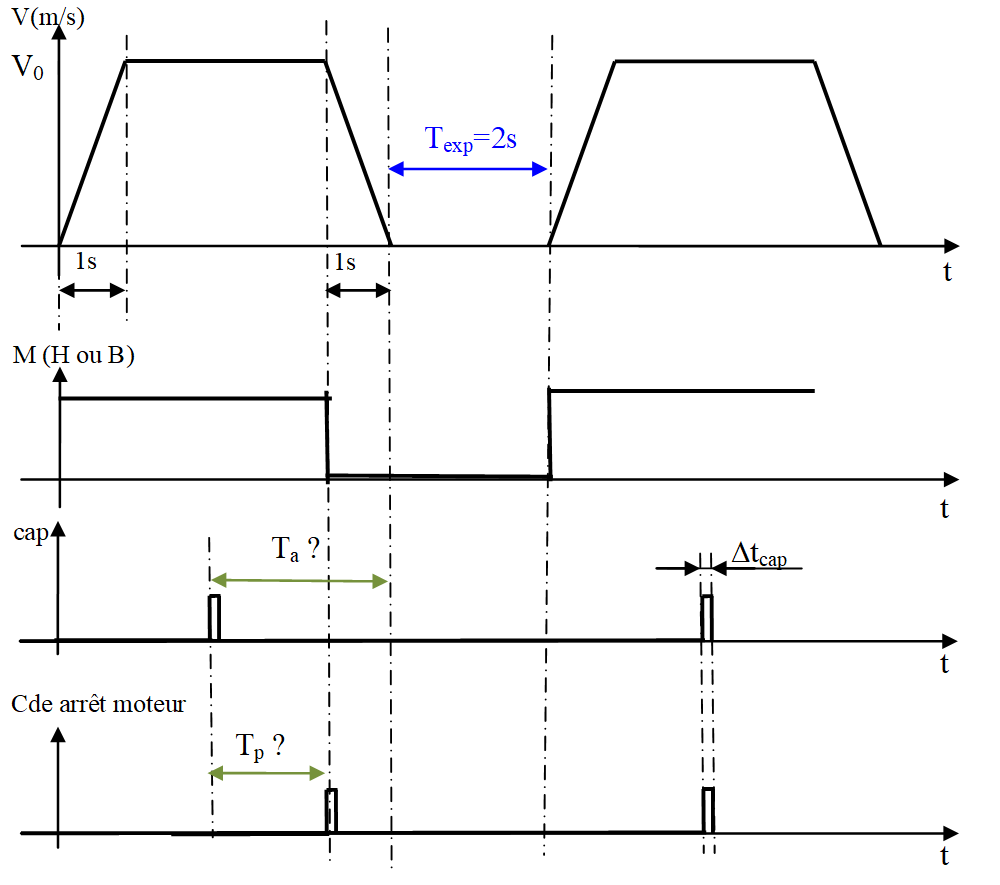
\includegraphics[width=0.7\linewidth]{img/fig07}
\end{center}
	\caption{Cycle de commande en fonctionnement normal}
	\label{fig07}
\end{figure}

\question{Déterminer le temps $T_a$ pour parcourir la distance $\frac{d}{2}$ en tenant compte de la phase de décélération.}

\question{En déduire la temporisation $T_p$ à programmer pour déclencher la décélération sur le variateur.}


\section{Étude de la fonction : \og tendre l'affiche \fg}

Au cours de l'enroulement du bandeau d'affiches sur un des rouleaux il faut éviter que l'affiche ne se plisse (problème de lecture de l'affiche par les passants) ou ne se déchire.

La tension $T_{aff}$ dans l'affiche est alors fixée par le constructeur dans l'intervalle suivant :
\begin{center}
$30N\leq T_{aff} \leq50N$
\end{center}

L'objectif est de comparer différentes solutions mises en place par le constructeur pour assurer le bon niveau de tension dans le bandeau d'affiches.

\subsection{Analyse de la solution 1 (solution à un seul moteur) (brevet N° FR 77 39575 année 1977)}

Lors des premières années de développement des panneaux d'affichage déroulant, une solution à un seul moteur a été développée.

Cette solution est décrite par une vue latérale sur le document annexe 5.

Elle est composée des éléments suivants :
\begin{itemize}
 \item un moteur,
 \item une transmission par chaîne,
 \item un contrepoids,
 \item un système de compensation.
\end{itemize}

\question{Dans quel sens (horaire ou trigonométrique) doit tourner la poulie motrice pour que le bandeau d'affiches s'enroule sur le rouleau haut ?}

\question{Quel élément du système permet d'assurer la tension dans le bandeau d'affiches ?}

\newpage

Cette solution a été rapidement abandonnée par le constructeur au profit d'une solution à deux moteurs.

\question{Énoncer deux raisons qui pourraient expliquer l'abandon de cette technologie.
Vous pourrez vous aider du document annexe 4 (brevet FR 2 659 161) décrivant la solution à deux moteurs.}

\subsection{Analyse de la solution à deux motorisations à commande alternée.}

Cette solution peut être décrite par le schéma simplifié suivant :

\begin{figure}[!h]
\begin{center}
	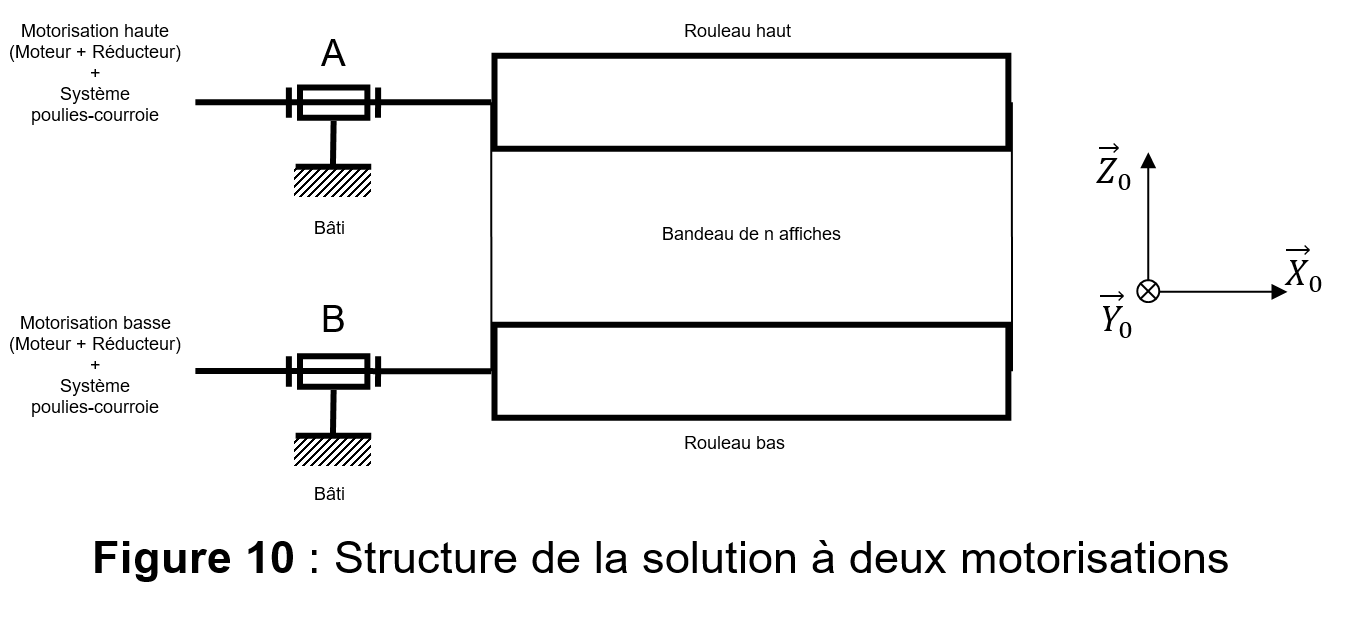
\includegraphics[width=0.8\linewidth]{img/fig10}
\end{center}
	\caption{Structure de la solution à deux motorisations}
	\label{fig10}
\end{figure}

Dans un premier temps, on utilise deux groupes motoréducteurs identiques.

Le fonctionnement de ce système est décrit par le tableau suivant :

\begin{center}
\begin{table}[!h]
\begin{tabular}{|c|c|c|}
\hline
& Motorisation haute	& Motorisation basse \\
\hline
Enroulement sur rouleau haut	 & Alimentée & Non alimentée \\
\hline
Enroulement sur rouleau bas & Non alimentée & Alimentée \\
\hline
\end{tabular}
\end{table}
\end{center}

Au cours de l'enroulement du bandeau d'affiches sur un rouleau, l'ensemble des pièces est donc entraîné par un seul moteur. 

Pour garantir en permanence une tension suffisante dans l'affiche même en régime établi, on décide d'implanter des organes de friction (frottement sec) au niveau de chaque liaison pivot entre chaque rouleau et le bâti.

Pendant l'enroulement sur le rouleau haut, l'action mécanique de chaque organe de friction sur chacun des rouleaux bas et haut peut être modélisée par le torseur suivant dans lequel $C_{fr}$ désigne le couple de frottement :

$\left\{T_{(Frott:bati\rightarrow rouleau\ haut)}\right\}=\left\{\begin{array}{c}
\overrightarrow{0} \\ -C_{fr}.\overrightarrow{X_0}\end{array}\right\}_A$ avec $C_{fr}>0$

$\left\{T_{(Frott:bati\rightarrow rouleau\ bas)}\right\}=\left\{\begin{array}{c}
\overrightarrow{0} \\ -C_{fr}.\overrightarrow{X_0}\end{array}\right\}_B$ avec $C_{fr}>0$

Pour l'étude, on propose alors le schéma détaillé suivant :
 
 \begin{figure}[!h]
\begin{center}
	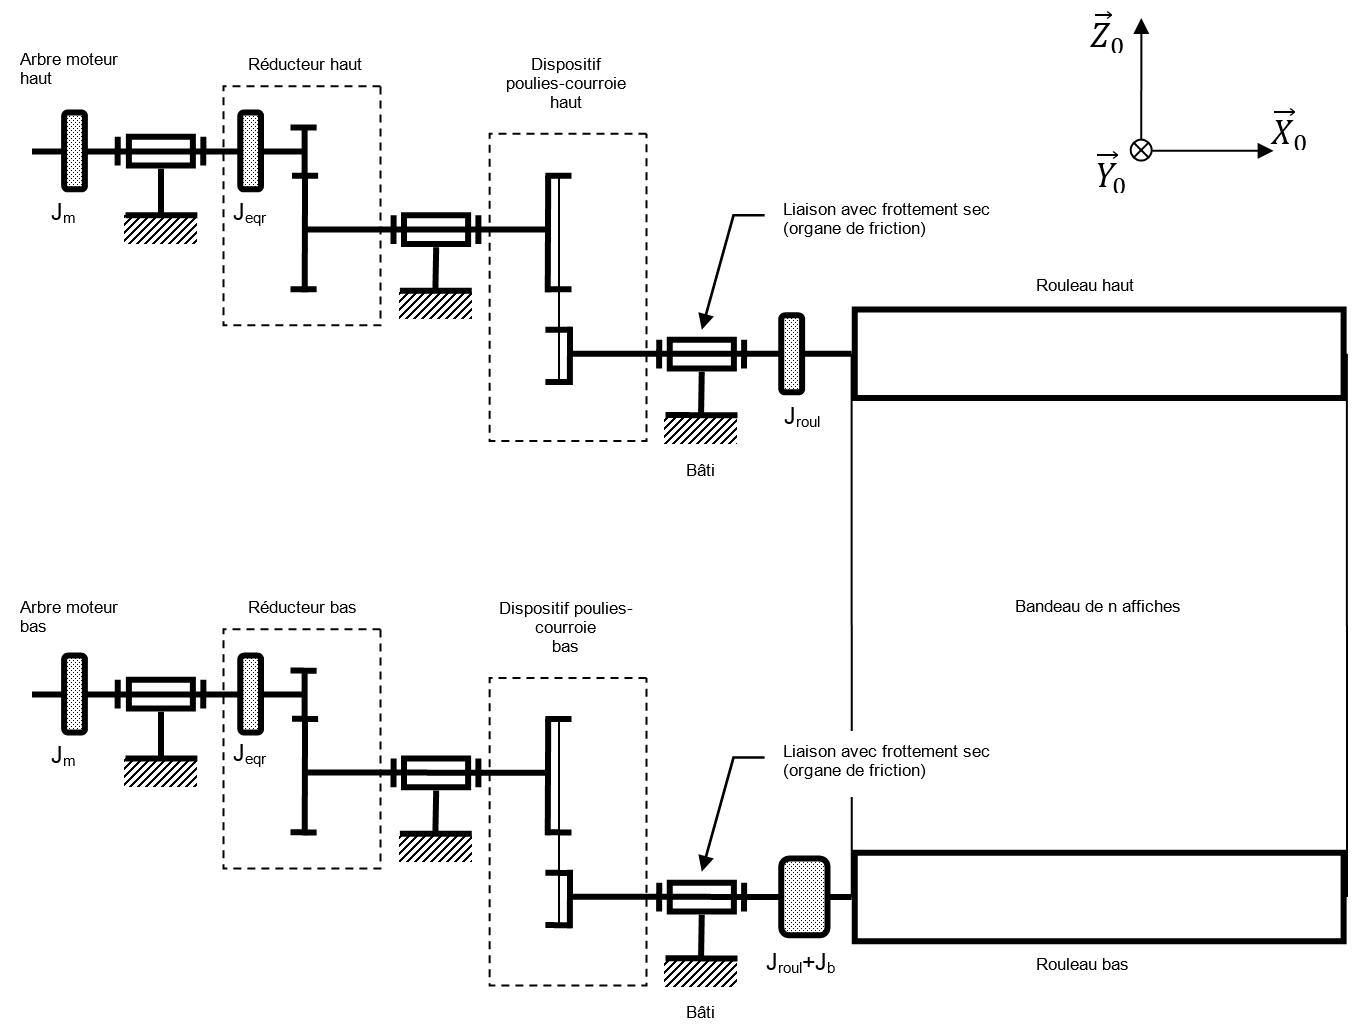
\includegraphics[width=0.8\linewidth]{img/fig11}
\end{center}
	\caption{Modèle retenu pour l'étude}
	\label{fig11}
\end{figure}

\textbf{Hypothèses :}
\begin{itemize}
 \item le référentiel $R_0$ lié au bâti 0 est galiléen,
 \item initialement le bandeau d'affiches est entièrement enroulé sur le rouleau bas,
 \item on étudie l'enroulement du bandeau sur le rouleau haut,
 \item les rayons des rouleaux sont supposés constants durant l'enroulement du bandeau sur le rouleau haut (les deux rouleaux tournent à la même vitesse pendant l'enroulement du bandeau),
 \item l'effet de la pesanteur est négligé face aux autres actions mécaniques,
 \item les liaisons sont supposées parfaites,
 \item les inerties des pièces des dispositifs poulies-courroie sont négligées,
 \item les courroies sont inextensibles et sans masse,
 \item le bandeau d'affiches est inextensible,
 \item la partie du bandeau d'affiches située entre les deux rouleaux (partie non enroulée) est sans masse.
\end{itemize}

~\

On appelle :
\begin{itemize}
 \item $am$ : les arbres moteur des transmissions haute et basse,
 \item $aer$ : les arbres d'entrée des réducteurs haut et bas,
 \item $asr$ : les arbres de sortie des réducteurs haut et bas,
 \item $roul$ : les rouleaux haut et bas.
\end{itemize}

~\

On note :
\begin{itemize}
 \item $J_{roul}$ : le moment d'inertie d'un rouleau vide par rapport à son axe,
 \item $J_m$ : le moment d'inertie de l'arbre moteur par rapport à son axe,
 \item $J_{eqr}$ : le moment d'inertie équivalent du réducteur ramené sur son arbre d'entrée,
 \item $J_b$ : le moment d'inertie du bandeau d'affiches par rapport à l'axe d'un rouleau lorsque le bandeau d'affiches est entièrement enroulé sur le dit rouleau,
 \item $\Omega_{roul}$ : la vitesse angulaire du rouleau autour de son axe par rapport à $R_0$,
 \item $\Omega_m$ : la vitesse angulaire de l'arbre moteur autour de son axe par rapport à $R_0$,
 \item $\Omega_{asr}$ : la vitesse angulaire de l'arbre de sortie du réducteur autour de son axe par rapport à $R_0$,
 \item $k_r$ : le rapport de transmission du réducteur:
 $k_r=\frac{\Omega_{asr}}{\Omega_{aer}}=\frac{\Omega_{asr}}{\Omega_m}$,
 \item $k_{pc}$ : le rapport de transmission du dispositif poulies-courroie,
$k_{pc}=\frac{\Omega_{roul}}{\Omega_{asr}}$,
 \item $C_m$ : le couple exercé sur l'arbre moteur par le stator du moteur alimenté.
\end{itemize}

\question{Donner l'expression de la vitesse linéaire de l'affiche en régime établi $V_0$ en fonction de $\Omega_m$, $k_r$, $k_{pc}$ et du rayon d'enroulement $R$ du bandeau sur le rouleau.}

~\

Pendant la phase d'accélération du bandeau d'affiche (voir figure \ref{fig03}), la vitesse de défilement du bandeau est variable. Elle est notée $V(t)$. L'accélération linéaire du bandeau est constante. Elle est notée $\gamma$.

\question{Donner l'expression de l'accélération linéaire de l'affiche $\gamma$ en fonction de $k_r$, $k_{pc}$, du rayon d'enroulement $R$ et de l'accélération angulaire de l'arbre moteur notée $\dot{\Omega}_m$.}

%~\
%
%Pour déterminer la tension dans l'affiche, on propose de se ramener au modèle équivalent suivant :
%\begin{figure}[!h]
%\begin{center}
%	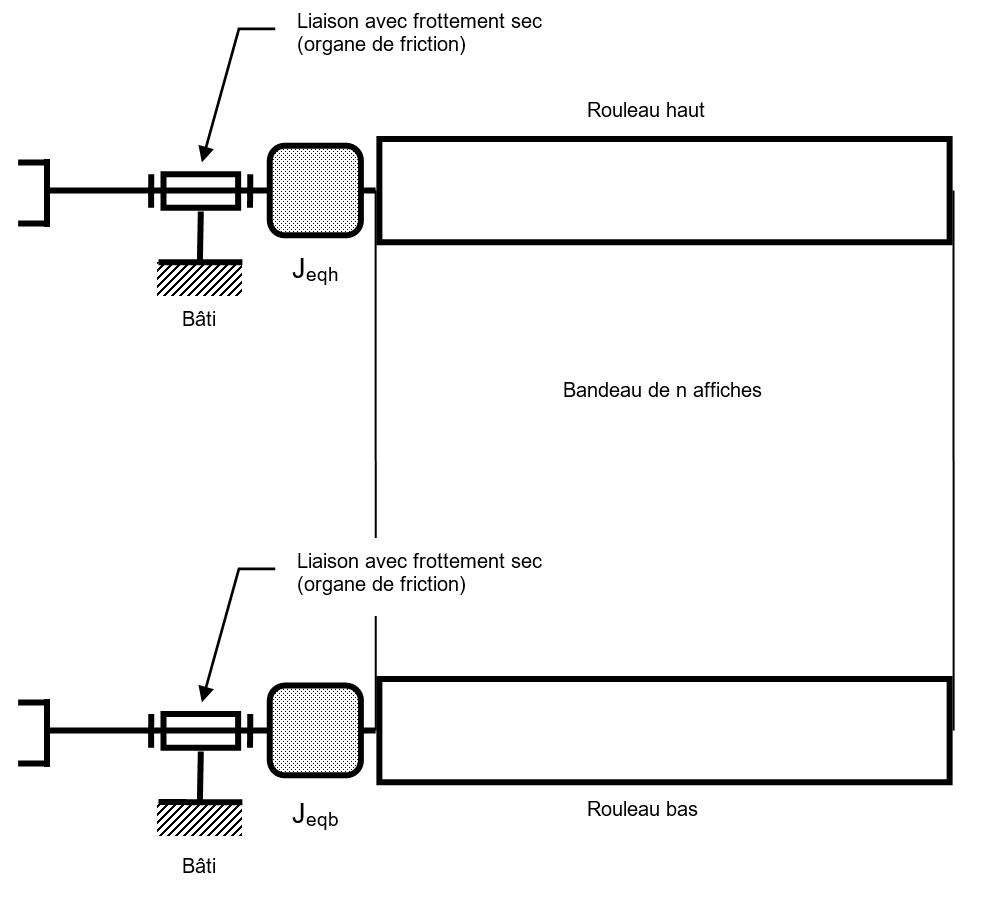
\includegraphics[width=0.7\linewidth]{img/fig12}
%\end{center}
%	\caption{Nouveau modèle retenu pour l'étude}
%	\label{fig12}
%\end{figure}

%On note :
%\begin{itemize}
% \item $J_{eqh}$ : le moment d'inertie équivalent de toute la chaîne de transmission haute ramené sur le rouleau haut,
% \item $J_{eqb}$ : le moment d'inertie équivalent de toute la chaîne de transmission basse ramené sur le rouleau bas.
%\end{itemize}
%
%\question{En utilisant la figure 11, exprimer en fonction de $\Omega_{roul}$, des différents moments d'inertie ($J_{roul}$, $J_m$, $J_{eqr}$, $J_b$) et de $k_r$ et $k_{pc}$, l'énergie cinétique T(S_bas?0) dans son mouvement par rapport à R_0 de l'ensemble S_bas formé par :
%	l'arbre moteur bas ;
%	l'arbre d'entrée bas du réducteur ;
%	l'arbre de sortie bas du réducteur ;
%	les arbres d'entrée et de sortie du dispositif poulies-courroie bas ;
%	le rouleau bas sur lequel est entièrement enroulé le bandeau d'affiches.}
%	
%En déduire l'expression du moment d'inertie équivalent J_eqb ramenée sur le rouleau bas.
%Calculer J_eqb si J_m=120 kg.?mm?^2, J_eqr=1,5 kg.?mm?^2 et (J_roul+J_b )=161500 kg.?mm?^2.

%On cherche maintenant la tension dans l'affiche $T_aff$ (effort exercé par la partie haute du bandeau s'enroulant sur le rouleau supérieur sur la partie basse du bandeau se déroulant du rouleau inférieur).
%
%L'action mécanique décrivant $T_{aff}$ est modélisée par le torseur suivant : \\
%\begin{center}
%$\left\{T_{(bandeau\ haut \rightarrow bandeau\ bas)}\right\}=\left\{\begin{array}{c}T_{aff}\cdot \overrightarrow{Z_0} \\ \overrightarrow{0}\end{array} \right\}_K$
%\end{center}
%
%Le modèle utilisé est le suivant :
%
%\begin{figure}[!h]
%\begin{center}
%	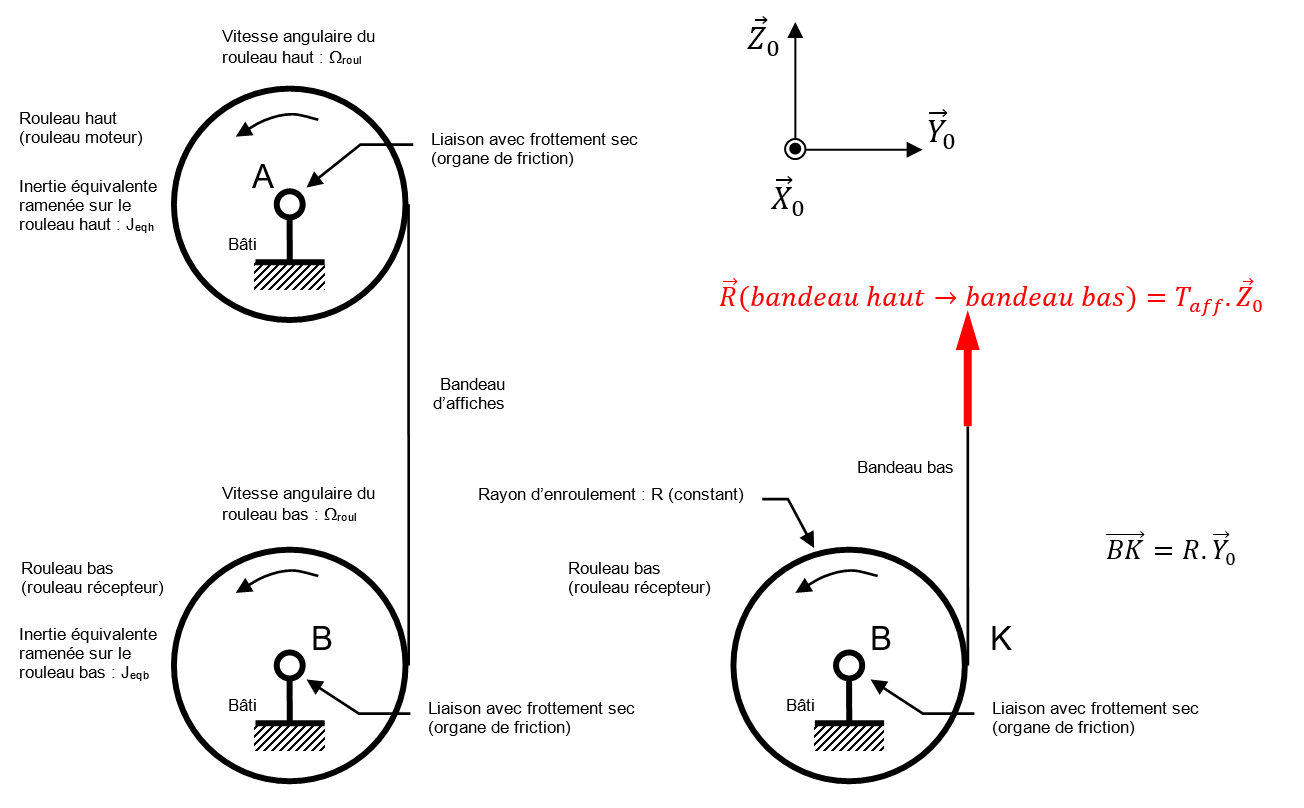
\includegraphics[width=0.8\linewidth]{img/fig13}
%\end{center}
%	\caption{Modèle pour l'analyse de la tension dans l'affiche}
%	\label{fig13}
%\end{figure}


%Détermination de la tension dans l'affiche en régime établi (vitesse linéaire de défilement du bandeau V_0)
%Appliquer le théorème du moment résultant (Principe Fondamental de la Statique) à l'ensemble ? = {rouleau bas + bandeau bas} selon l'axe (B,X ?_0 ) pour déterminer la relation liant la tension dans l'affiche T_aff, le couple de frottement C_fr et le rayon d'enroulement R.
%Calculer la valeur de C_fr si on souhaite fixer la tension T_aff dans l'affiche à 40 N avec un rayon d'enroulement R=76 mm.
%
%Pour la suite de l'étude, on fixe le couple de frottement à C_fr=3 N.m.
%
%Détermination de la tension dans l'affiche en régime transitoire (phase d'accélération du bandeau)
%Appliquer le théorème du moment dynamique à l'ensemble ? = {rouleau bas + bandeau bas}  selon l'axe (B,X ?_0 )  dans son mouvement par rapport au repère galiléen R_0 pour déterminer la relation liant la tension dans l'affiche T_aff, l'accélération linéaire de l'affiche ?, l'inertie équivalente J_eqb, le rayon d'enroulement R et le couple de frottement C_fr.
%Calculer la tension dans l'affiche T_aff si ?=1 m.s^(-2),  k_r=1?19,5, k_pc=2, J_eqb=173.?10?^3  kg.?mm?^2, R=76 mm et C_fr=3 N.m.
%La tension dans l'affiche en régime transitoire respecte-t-elle le cahier des charges fonctionnel (fonction FP12) ?
%Le constructeur a donc mis en place une nouvelle solution pour assurer le bon niveau de tension dans l'affiche.
%Cette solution est décrite dans le brevet FR2659161 déposé par JC DECAUX. Elle est basée sur : 
%	un moteur haut commandé en vitesse pour assurer le déplacement du bandeau d'affiches ;
%	un moteur bas commandé en couple afin d'assurer la tension du bandeau d'affiches.
%La solution retenue utilise un moteur asynchrone pour assurer le déplacement du bandeau et un moteur à courant continu pour assurer la tension des affiches (voir diagramme FAST annexe 3).
%
%Analyse du comportement de la solution 2 (Brevet FR 2659161 de septembre 1992) : association MCC et MAS
%Réglage de la vitesse du moteur asynchrone
%Le moteur asynchrone est commandé par un variateur de type U?f constant. La vitesse nominale de défilement d'un affiche est de 1 m.s^(-1). Le moteur utilisé est un motoréducteur réf W10DT56L4.
%Le but de l'étude est de vérifier le dimensionnement du moteur asynchrone et de régler la fréquence du variateur afin de répondre au mieux au cahier des charges.
%Dans cette étude, on s'intéressera au fonctionnement à vitesse constante.
%On notera :
%	? : la vitesse angulaire exprimée en rad/s ;
%	N : la fréquence de rotation exprimée en tr/min.
%Compte tenu de la tension dans l'affiche, on obtient un couple moteur C_m=0,28 N.m à une vitesse angulaire ?_m=139 rad.s^(-1).
%
%Déterminer la puissance P_m nécessaire en régime permanent.

%Les caractéristiques du moteur lorsqu'il est alimenté sur un réseau 50 Hz sont les suivantes :
%P_N : puissance nominale sur l'arbre du moteur 		120 W
%N_N : vitesse nominale en sortie d'arbre			1300 tr.?min?^(-1)
%I_N : courant nominal à vitesse nominale			0,8 A
%cos?? : facteur de puissance				0,68
%I_D?I_N  : courant au démarrage/courant nominal		2,6
%C_N : couple nominal					0,88 N.m
%C_max?C_N  : couple maximal/couple nominal			1,9  
%
%A partir des caractéristiques du moteur et de la réponse à la question précédente, montrer que le moteur est largement surdimensionné.
%
%En réalité, le rendement de la transmission n'est pas égal à 1. En conséquence, la valeur du couple électromagnétique en fonctionnement normal est C_maff=0,3 N.m
%?
%On rappelle que l'expression du couple électromagnétique pour un moteur asynchrone est :
%C_m1=(2.C_max)/(g_0/g+g/g_0 )	C_max : couple maximal du moteur. 
%g : glissement
%g_0 : glissement pour le couple C_max
%Donner l'expression de g en fonction de la vitesse angulaire ?_m et la vitesse de synchronisme ?_s.
%Donner l'expression de ?_s en fonction de ? (pulsation du réseau) et de p (nombre de paire de pôles) puis déterminer ?_s et N_s lorsque le moteur est alimenté par un réseau triphasé à une fréquence de 50 Hz. Compte tenu des caractéristiques du moteur, montrer que le nombre de paires de pôles de la machine est égal à 2.
%A partir des données du constructeur, déduire la valeur du glissement au point de fonctionnement nominal g_N.
%Calculer la valeur g_0 à partir de l'expression du couple moteur C_m1. 
%Tracer l'allure de la caractéristique C_m en fonction de g (pour 0<g<1) en indiquant les valeurs numériques de C_N, g_N, C_max, g_0 sur la courbe. Précisez la zone de fonctionnement stable du moteur.
%Le système fonctionnant  à une valeur de couple C_m1=C_maff=0,3 N.m donc inférieure à C_N, montrer que l'expression du couple moteur peut se mettre sous la forme C_m1=2.g/g_0 .C_max et en déduire la valeur du glissement g_aff pour le couple C_maff .
%Montrer que l'expression du couple peut s'exprimer par : C_m1=?.(?_s-?_m )   Précisez l'expression de  ?.
%On sait que dans le modèle équivalent du moteur asynchrone on a : 
%C_max=(3pV^2)/(2l_2 ?²)	et	g_0=R_2/(l_2 ?)   	 
%V : la tension simple aux bornes d'un enroulement, 
%l2 : l'inductance secondaire ramenée au primaire 
%R2 : la résistance rotorique secondaire ramenée au primaire	
%Justifier que ?  est constant lorsque l'on commande le moteur avec un variateur de vitesse à V?f constant.
%Dans la suite du problème, on prendra  ?=0,0453 N.m.s.?rad?^(-1).
%Sachant que le moteur doit tourner à la vitesse de ?_m=139 rad.s^(-1) avec un couple C_maff=0,3 N.m pour respecter le cahier des charges, quelle devra être la vitesse de synchronisme ?_s ? En déduire la valeur de la fréquence f_v à programmer dans le variateur de vitesse du moteur pour respecter le cahier des charges.
%

\subsubsection{Étude de l'asservissement en couple du moteur à courant continu}

Le but de cette étude est de vérifier les comportements statique et dynamique du système assurant la fonction \og tendre l'affiche \fg et de définir le type de correcteur le mieux approprié à cette application.

Le moteur haut est un moteur asynchrone qui assure le défilement des affiches. Le moteur bas est un moteur à courant continu à aimant permanent asservi en couple grâce à un variateur. Il assure la tension des affiches.

~\

On rappelle les équations du moteur en négligeant l'inductance de l'induit :

$\left\{\begin{array}{l}
E(t)=k_e.\Omega_m (t) \\
C_m(t)=k_c.i(t) \\
V_a(t)=R_a.i(t)+E(t)\\
J_{mc}.\frac{d\Omega_m(t))}{dt}=C_m(t)-C_r(t)
\end{array}\right.$

~\

Avec:
\begin{itemize}
 \item $k_c$ : constante de couple,
 \item $k_e$ : constante de f.e.m. On posera $k_e=k_c=k$,
 \item $R_a$ : résistance d'induit,
 \item $J_{mc}$ : moment d'inertie ramené sur l'arbre du moteur,
 \item $C_r$ : couple résistant,
 \item $C_m$ : moment du couple moteur,
 \item $V_a$ : tension appliquée aux bornes de l'induit, 
 \item $\Omega_m$ : vitesse angulaire de l'arbre du moteur,
 \item $i$ : courant d'induit.
\end{itemize}

\newpage

\question{Déterminer les transformées de Laplace de ces différentes expressions.}

~\

Le moteur asservi se présente sous la forme suivante où la partie en pointillé représente le modèle du moteur à courant continu :

\begin{figure}[!h]
\begin{center}
	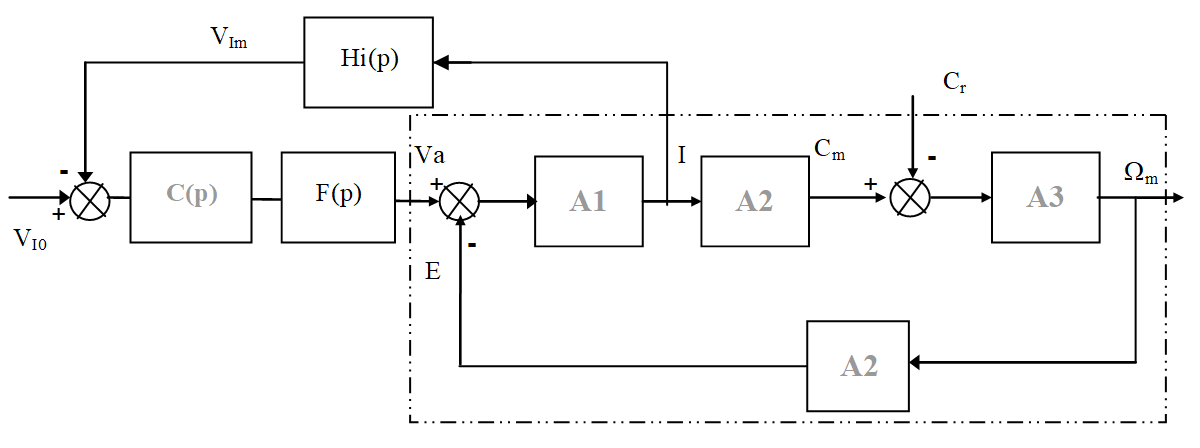
\includegraphics[width=0.6\linewidth]{img/fig14}
\end{center}
	\caption{Schéma bloc du moteur asservi}
	\label{fig14}
\end{figure}
 
\begin{itemize}
 \item $V_{I0}$ représente la consigne de courant donc de couple,
 \item $F(p)$ représente la fonction de transfert du hacheur commandant le moteur. Elle est supposée constante $F(p)=F_0$,
 \item $C(p)$ le correcteur associé au hacheur,
 \item On appelle  $H(p)=C(p).F(p)$,
 \item $H_i(p)$ représente le capteur de courant.
\end{itemize}

\question{Déterminer les expressions des différents blocs $A1$, $A2$, $A3$ associés au modèle du moteur à courant continu.}

~\

Le système commandé en couple peut donc se mettre sous la forme suivante :
 
\begin{figure}[!h]
\begin{center}
	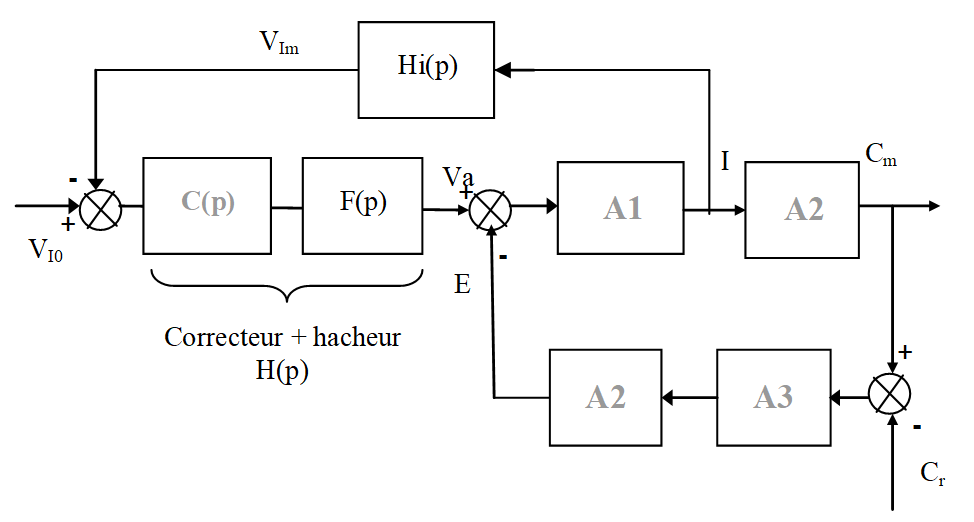
\includegraphics[width=0.6\linewidth]{img/fig15}
\end{center}
	\caption{Schéma bloc de l'asservissement en couple}
	\label{fig15}
\end{figure}

\question{Exprimer $C_m$ en fonction de $V_{I0}$, $C_r$ et des fonctions de transfert.}

\newpage

$C_r$ représente le couple résistant de l'ensemble affiches, rouleaux, réducteurs et moteur asynchrone d'entraînement haut.

\textbf{Hypothèses :}
\begin{itemize}
 \item 	on néglige toutes les pertes associées aux différents éléments de la chaine de transmission que l'on suppose rigide,
 \item on suppose que le rapport de réduction du moteur asynchrone est le même que celui du moteur à courant continu. De ce fait, et compte tenu que l'épaisseur du papier est négligeable, on peut considérer que les deux machines tournent à la même vitesse angulaire,
 \item on a donc $C_r=-C_{m1}$.
\end{itemize} 

~\

D'après les résultats de l'exercice précédent, on obtient donc :\\
$C_r=-\lambda.(\Omega_s-\Omega_m)=\lambda.(\Omega_m-\Omega_s)$.

~\

On obtient alors le schéma complet de l'ensemble des deux machines :

\begin{figure}[!h]
\begin{center}
	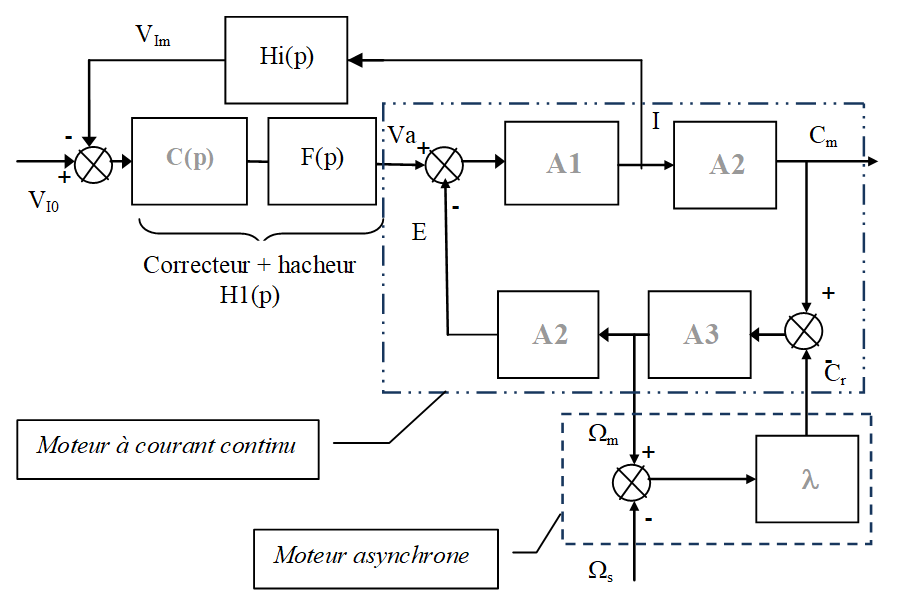
\includegraphics[width=0.6\linewidth]{img/fig16}
\end{center}
	\caption{Schéma bloc de l'ensemble des deux machines}
	\label{fig16}
\end{figure}

\question{Déterminer l'expression de $C_m$ en fonction des différents éléments et de $V_{I0}$ et $\Omega_s$.}

\question{Proposer une structure de hacheur permettant de commander le moteur à courant continu afin de fonctionner dans les deux sens de rotation tout en assurant un couple quasi-constant. Utiliser pour cela les deux composants suivants.}

\begin{center}
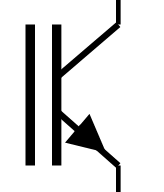
\includegraphics[width=0.1\linewidth]{img/transistor} \hspace{1cm} 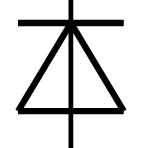
\includegraphics[width=0.1\linewidth]{img/diode} 
\end{center}

\newpage

\subsubsection{Mesure du courant image du couple moteur}

La mesure du couple moteur se fait par la mesure du courant grâce à un capteur à effet Hall qui délivre une tension $V_{im}$.

On obtient une tension $V_{im}(1V.A^{-1})$ image du courant $I_m$ dans le moteur.

L'allure de l'image du courant est la suivante :

\begin{figure}[!h]
\begin{minipage}{0.5\linewidth}
\begin{center}
	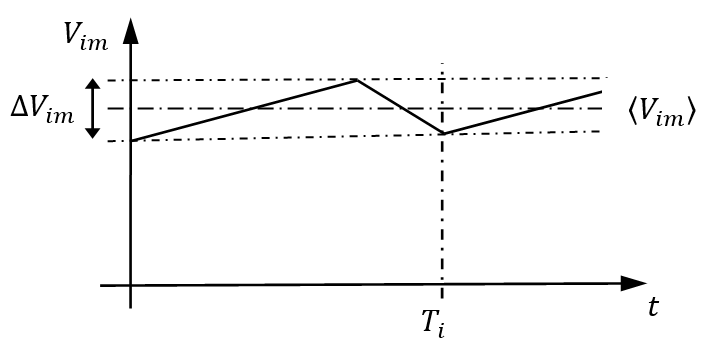
\includegraphics[width=0.9\linewidth]{img/fig17}
\end{center}
	\caption{Image du courant $I_m$}
	\label{fig17}
\end{minipage}\hfill
\begin{minipage}{0.45\linewidth}
\begin{itemize}
 \item $\left\langle  V_im\right\rangle$ tension image du courant moyen,
 \item $V_{im}$ tension image de l'ondulation du courant,
 \item $T_i=0,5ms$.
\end{itemize}
\end{minipage}
\end{figure}

On désire obtenir l'image du courant moyen avec une atténuation de l'ondulation relative $\frac{\Delta V_{im}}{\left\langle V_im \right\rangle}$ d'au moins 40dB afin d'obtenir une valeur moyenne sans perturbation pour un asservissement correct. Le but est de dimensionner les composants du filtre passif.

Pour cela on utilise la structure suivante dont l'étude sera menée avec la représentation complexe (on rappelle que l'impédance d'un condensateur idéal est notée $z_c=\frac{1}{j.C.\omega}$).
 
\begin{figure}[!h]
\begin{center}
	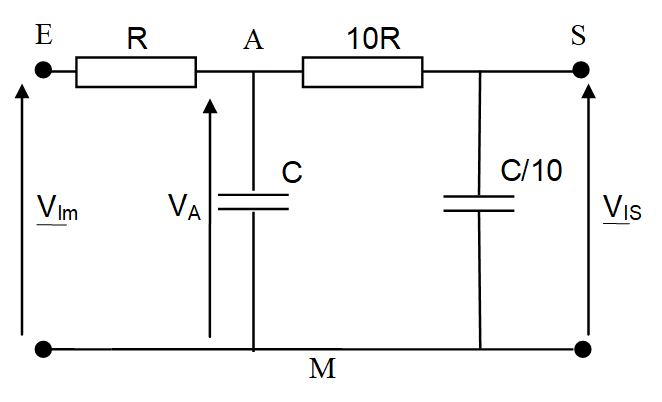
\includegraphics[width=0.6\linewidth]{img/fig18}
\end{center}
	\caption{Structure du filtre passif}
	\label{fig18}
\end{figure}

\question{Quel type de filtre permet de garder la composante continue et d'atténuer l'ondulation ?}

\question{Exprimer la tension $V_A$ en fonction des tensions $V_{is}$ et $V_{im}$ et les différents composants.}

\question{Exprimer $V_{is}$ en fonction de $V_A$. En déduire l'expression de la fonction de transfert et montrer qu'elle se met sous la forme :\\
$\frac{V_{is}}{V_{im}}=\frac{1}{1+\alpha\cdot j\cdot\frac{\omega}{\omega_0}+\left(j\cdot\frac{\omega}{\omega_0}\right)^2}$ avec $\omega_0=\frac{1}{R\cdot C}$}

\question{On désire une atténuation de 40dB du fondamental $\omega_i$ du signal $V_{im}$. Compte tenu de la fréquence de ce signal calculer la valeur de la pulsation $\omega_0$.}

~\

On prendra $R=10k\Omega$ pour ne pas trop charger le capteur à effet Hall.

\question{En déduire la valeur de C.}

\subsection{Étude du comportement de la solution actuelle (solution 3)}

Pour une simplicité de la maintenance, la dernière solution retenue par JC Decaux consiste en l'utilisation de deux motoréducteurs asynchrones identiques associés à deux variateurs de vitesse.

Le réglage du couple moteur et donc de la tension des affiches se fait par réglage différentiel des vitesses de synchronisme des deux moteurs.

\begin{figure}[!h]
\begin{center}
	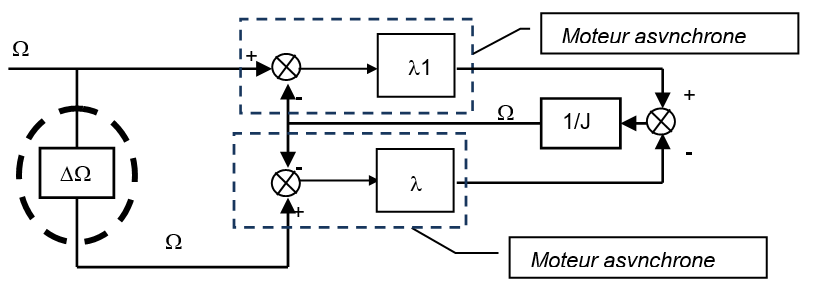
\includegraphics[width=0.6\linewidth]{img/fig19}
\end{center}
	\caption{Modèle de la solution 3}
	\label{fig19}
\end{figure}

\begin{figure}[!h]
\begin{minipage}{0.5\linewidth}
Lors d'une phase d'enroulement sur le rouleau haut (phase en montée), on obtient les caractéristiques $C(\Omega)$ ci-contre (M1 trait continu, M2 trait pointillé) :
\end{minipage}\hfill
\begin{minipage}{0.45\linewidth}
\begin{center}
	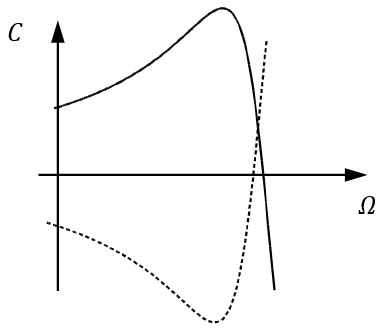
\includegraphics[width=0.45\linewidth]{img/fig20}
\end{center}
\end{minipage}
\caption{Caractéristiques Couple - Vitesse}
\label{fig20}
\end{figure}

Le but est de déterminer le réglage du différentiel de fréquence $\Delta f$ (donc $\Delta\Omega_s=\Delta_f\cdot \pi=\Omega_{s1}-\Omega_{s2}$) entre les deux variateurs afin d'obtenir un couple $C_m=0,3Nm$ permettant d'assurer la tension correcte des affiches.

Compte tenu du fait que les machines fonctionnent dans leur zone linéaire, les caractéristiques des machines dans le plan $C(\Omega)$ dans les deux phases de fonctionnement sont les suivantes :
 
\begin{figure}[!h]
\begin{center}
	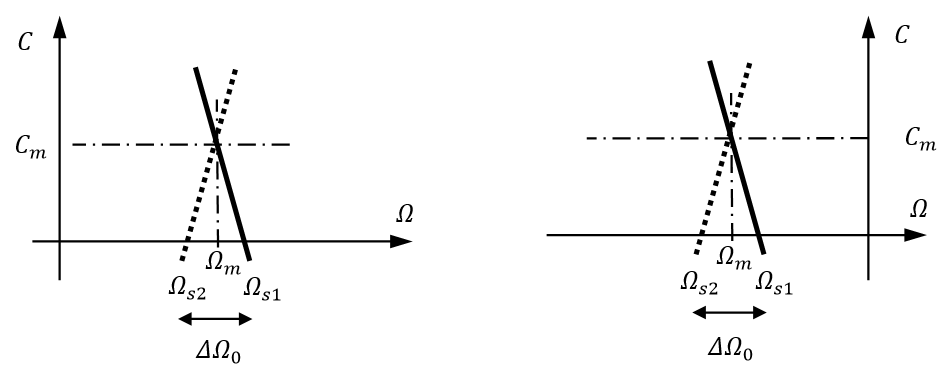
\includegraphics[width=0.4\linewidth]{img/fig21}
\end{center}
\caption{Caractéristiques des deux machines}
\label{fig21}
\end{figure}

\newpage

Ceux-ci fonctionnent dans la partie linéaire de leur caractéristique. En conséquence on obtient les équations suivantes :

\begin{minipage}{0.45\linewidth}
\begin{itemize}
 \item $C_m(t)=\lambda.\left(\Omega_{s1}-\Omega_m\right)$,
 \item $C_r(t)=\lambda.(\Omega_m-\Omega_{s2})$,
 \item $J_{mc}.\frac{d\Omega_m(t)}{dt}=C_m(t)-C_r(t)$
\end{itemize}
\end{minipage}
\begin{minipage}{0.45\linewidth}
\begin{itemize}
 \item $\lambda=0,05$ : coefficient du moteur,
 \item $J_{mc}$ : moment d'inertie ramené sur l'arbre du moteur 1,
 \item $C_r$ : moment du couple moteur 2 fonctionnant en couple résistant,
 \item $C_m$ : moment du couple moteur 1.
\end{itemize}
\end{minipage}

\question{Déterminer l'expression de l'équation différentielle du moteur. En déduire la vitesse $\Omega_m$ du moteur en régime permanent en fonction de $\Omega_{s1}$ et $\Omega_{s1}$.}

\question{Déterminer l'écart de pulsation $\Delta\Omega_s$ pour avoir un couple $C_m=0,3Nm$ en régime permanent de vitesse. En déduire $\Delta f$.}

\section{Étude de la fonction : \og guider le rouleau par rapport au châssis \fg}
 
L'objectif est de justifier la présence d'un dispositif de réglage permettant un enroulement correct du bandeau d'affiches et la présence d'une spécification géométrique sur le rouleau.
Le modèle retenu pour l'étude est le suivant :

\begin{figure}[!h]
\begin{center}
	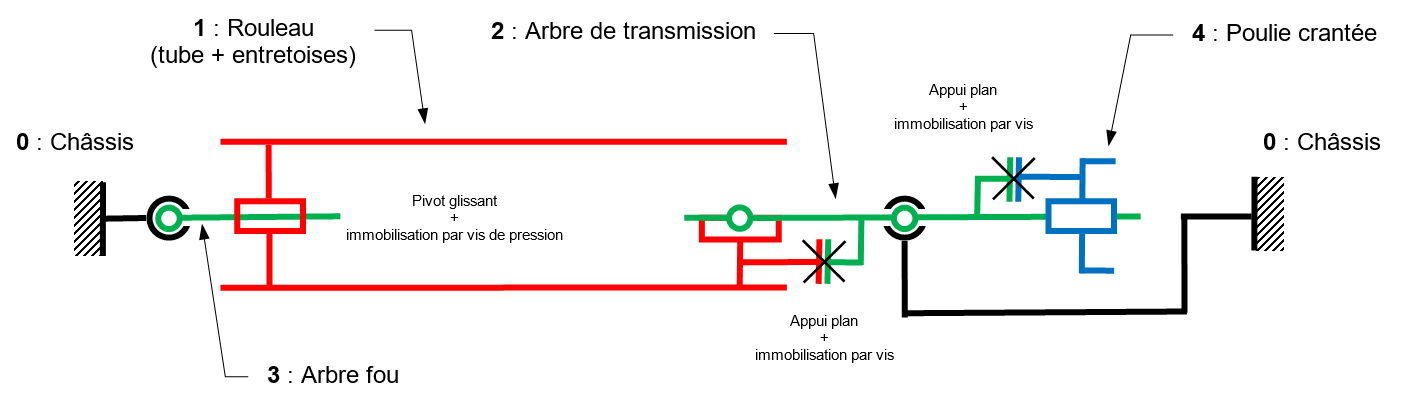
\includegraphics[width=0.9\linewidth]{img/fig22}
\end{center}
\caption{Modèle retenu pour le montage et l'entraînement d'un rouleau}
\label{fig22}
\end{figure}

L'entraînement du rouleau 1 est réalisé grâce une courroie crantée montée sur la poulie crantée 4 elle-même montée sur l'arbre de transmission 2.

\question{Déterminer le degré d'hyperstatisme $h$ de la liaison entre l'ensemble formé par le rouleau 1, l'arbre de transmission 2 et l'arbre fou 3 (qui sera considéré comme une classe d'équivalence) et le châssis 0.}

\question{Quelles sont les conséquences sur les conditions d'assemblage de ces trois pièces ?}

~\

\textbf{Remarque :} vous pourrez vous aider de croquis ou schémas.

\newpage

On souhaite étudier les conséquences d'écarts d'orientation et de position au niveau du châssis 0.

La prise en compte de ces écarts sur le châssis peut aboutir à la situation décrite par le modèle d'écart suivant :

\begin{figure}[!h]
\begin{center}
	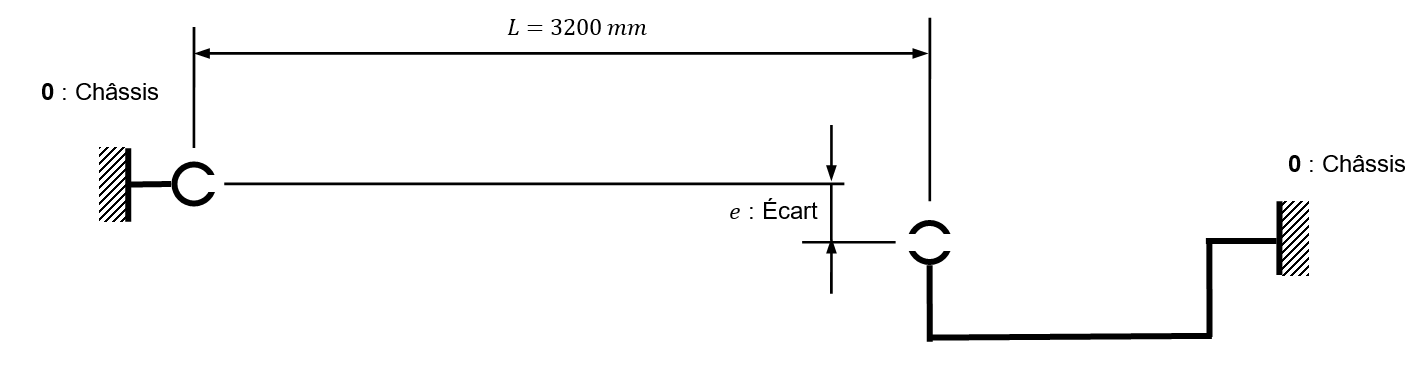
\includegraphics[width=0.6\linewidth]{img/fig23}
\end{center}
\caption{Modèle d'écart pour le châssis 0}
\label{fig23}
\end{figure}

Si on suppose que les pièces autres que le châssis sont sans défaut, l'assemblage avec le châssis donnera la situation suivante :

\begin{figure}[!h]
\begin{center}
	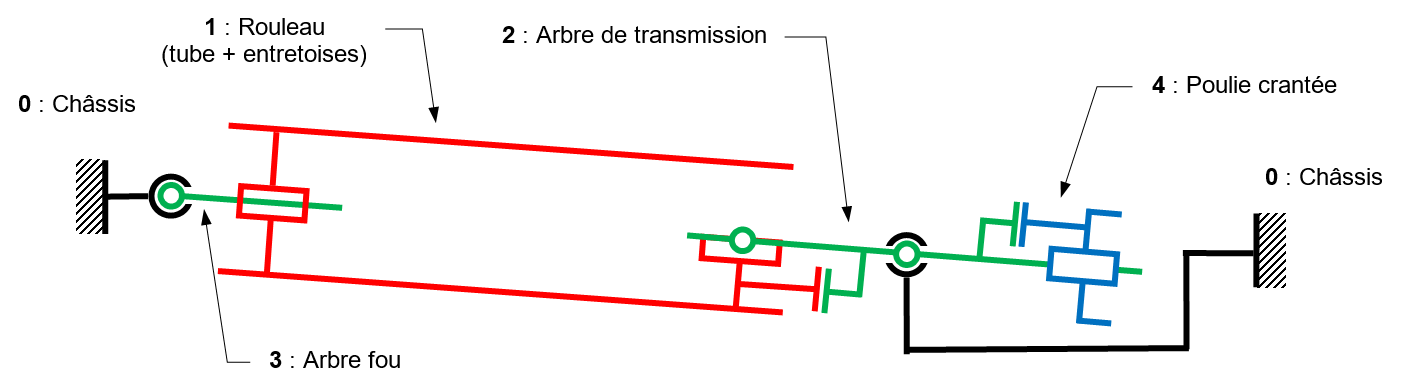
\includegraphics[width=0.6\linewidth]{img/fig24}
\end{center}
\caption{Modèle de l'assemblage avec châssis comportant un écart}
\label{fig24}
\end{figure} 

Les liaisons entre le châssis 0 et les arbres de transmission 2 et fou 3 sont assurées respectivement par des roulements à deux rangées de billes de type 2204 E 2RS et 2205 E 2RS.

Des caractéristiques de ces roulements sont données sur le document annexe 6.

\question{Les roulements utilisés sont-ils adaptés pour accepter cette situation ? Pourquoi ?}

\question{Quel problème risque-t-on de rencontrer au niveau de la transmission poulie-courroie ?}

Pour minimiser ce problème, on décide de modifier la solution de guidage du rouleau par rapport au châssis.

\question{Proposer un dispositif de réglage sous forme de schéma cinématique permettant d'annuler ce problème.}

~\

On s'intéresse maintenant plus particulièrement à la liaison entre le rouleau 1 et l'arbre fou 3.

Cette liaison est réalisée par deux portées cylindriques.

Étant donné la valeur du rapport « longueur du guidage / diamètre de l'arbre », on choisit d'adopter un nouveau modèle pour l'étude de la liaison entre le rouleau 1 et l'arbre fou 3.

\newpage

Ce modèle est constitué de deux liaisons pivots glissants :

\begin{figure}[!h]
\begin{center}
	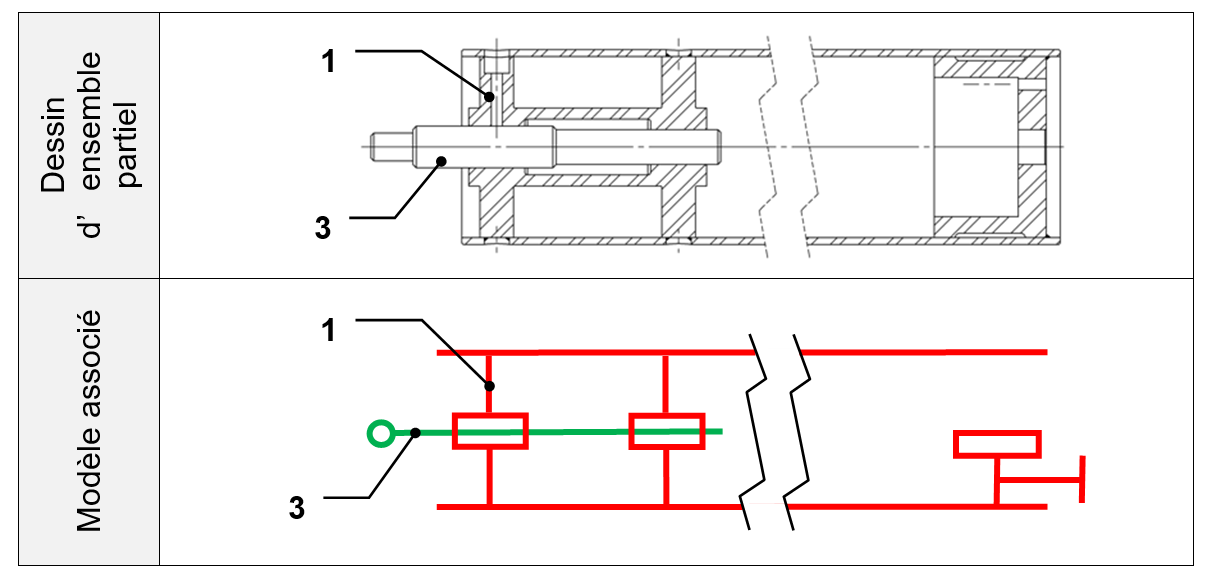
\includegraphics[width=0.6\linewidth]{img/fig25}
\end{center}
\caption{Assemblage rouleau - arbre fou (Dessin d'ensemble partiel - Modèle associé)}
\label{fig25}
\end{figure} 

\question{Déterminer le degré d'hyperstatisme de l'assemblage du rouleau 1 et l'arbre fou 3.}

~\

On s'intéresse maintenant au guidage entre l'arbre de transmission 2 et le châssis 0 et à la liaison entre l'arbre de transmission 2 et la poulie crantée 4.

Le document réponse (à rendre avec la copie) propose une mise en place des différents composants concernés.
On y voit notamment :
\begin{itemize}
 \item le rouleau 1,
 \item l'arbre de transmission 2 (formes à compléter),
 \item le roulement à deux rangées de billes de type 2204 E 2RS (roulement graissé à vie),
 \item la poulie crantée 4 (formes à compléter),
 \item le support de roulement (formes à compléter) fixé sur le montant du panneau d'affichage et assurant le guidage de la bague extérieur du roulement.
\end{itemize}

\question{Compléter la vue en coupe AA du document réponse.}

On représentera notamment :
\begin{itemize}
 \item les arrêts axiaux des bagues du roulement à billes,
 \item une solution démontable permettant la transmission du couple entre la poulie 4 et l'arbre de transmission 2,
 \item les formes des pièces à compléter,
 \item les tolérances arbre et alésage pour le montage des bagues du roulement à billes.
\end{itemize}

\newpage

~\

\vspace{10cm}

\begin{center}
\Huge{Annexes}
\end{center}

\newpage

\textbf{Annexe 1}

Caractéristiques techniques du produit actuel

Caractéristiques techniques du système :
\begin{itemize}
 \item panneau $8m^2$,
 \item déroulant vertical pour 2 à 7 affiches,
 \item détection des affiches par un capteur optique,
 \item rétro éclairage par 14 tubes fluorescents,
 \item alimentation électrique : 220V - 50Hz monophasé,
 \item matériel de classe I : protection différentielle de 30mA et mise à la terre,
 \item entraînement : deux moteurs asynchrones SEW Eurodrive associés à deux variateurs,
 \item automate programmable: Siemens S7-216,
 \item interface de dialogue avec l'automate: console Siemens TD200 ou système GSM Wacom,
 \item consommation : moins de 400W pour un système déroulant et 815W pour l'éclairage.
\end{itemize}

Caractéristiques techniques des affiches à utiliser :
\begin{itemize}
 \item support : Papier ou longue conservation (165 ou 190 $g.m^{-2}$),
 \item dimensions : 3130 x 2300 mm,
 \item épaisseur : 200$\mu m$,
 \item résistance à la traction : ISO 187:1990,
 \item accroche des affiches par système Zip Grip.
\end{itemize}

Cahier des charges de fonctionnement classique:
\begin{itemize}
 \item rampe d'accélération et de décélération : 1s,
 \item temps d'exposition d'une affiche : Tex = 2s à la montée et à la descente,
 \item temps d'exposition des affiches extrêmes : 4s,
 \item vitesse de défilement d'une affiche : $V_0=1m.s^{-1}$,
 \item effort de tension sur les affiches : entre 30N et 50N.
 \end{itemize}

\newpage

\textbf{Annexe 4}

\begin{center}
 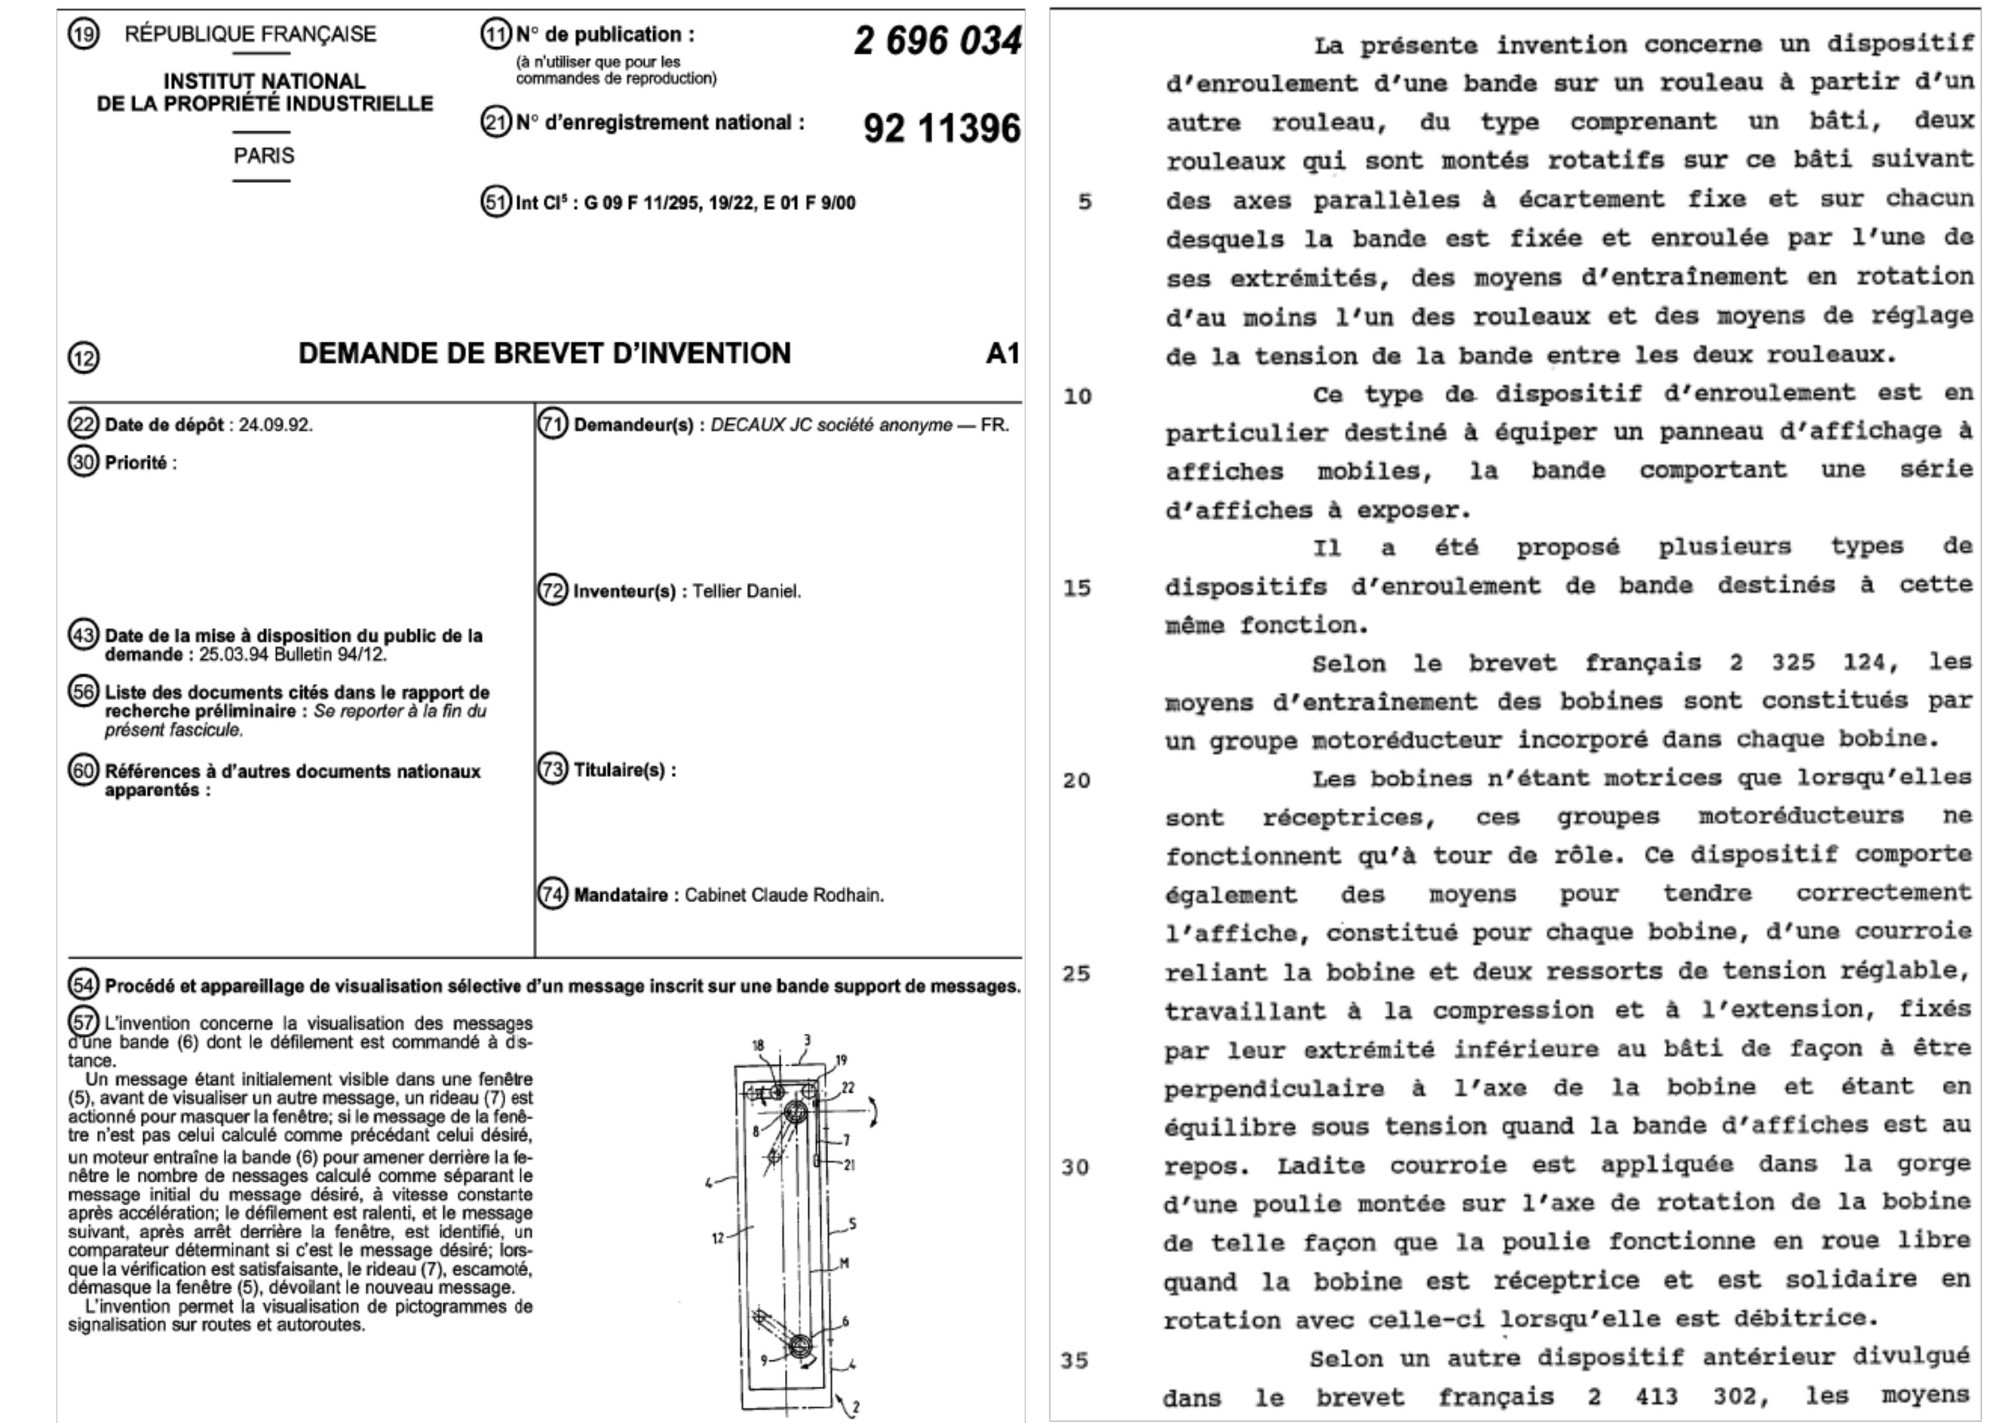
\includegraphics[width=0.9\linewidth]{img/annexe4_1}

~\

 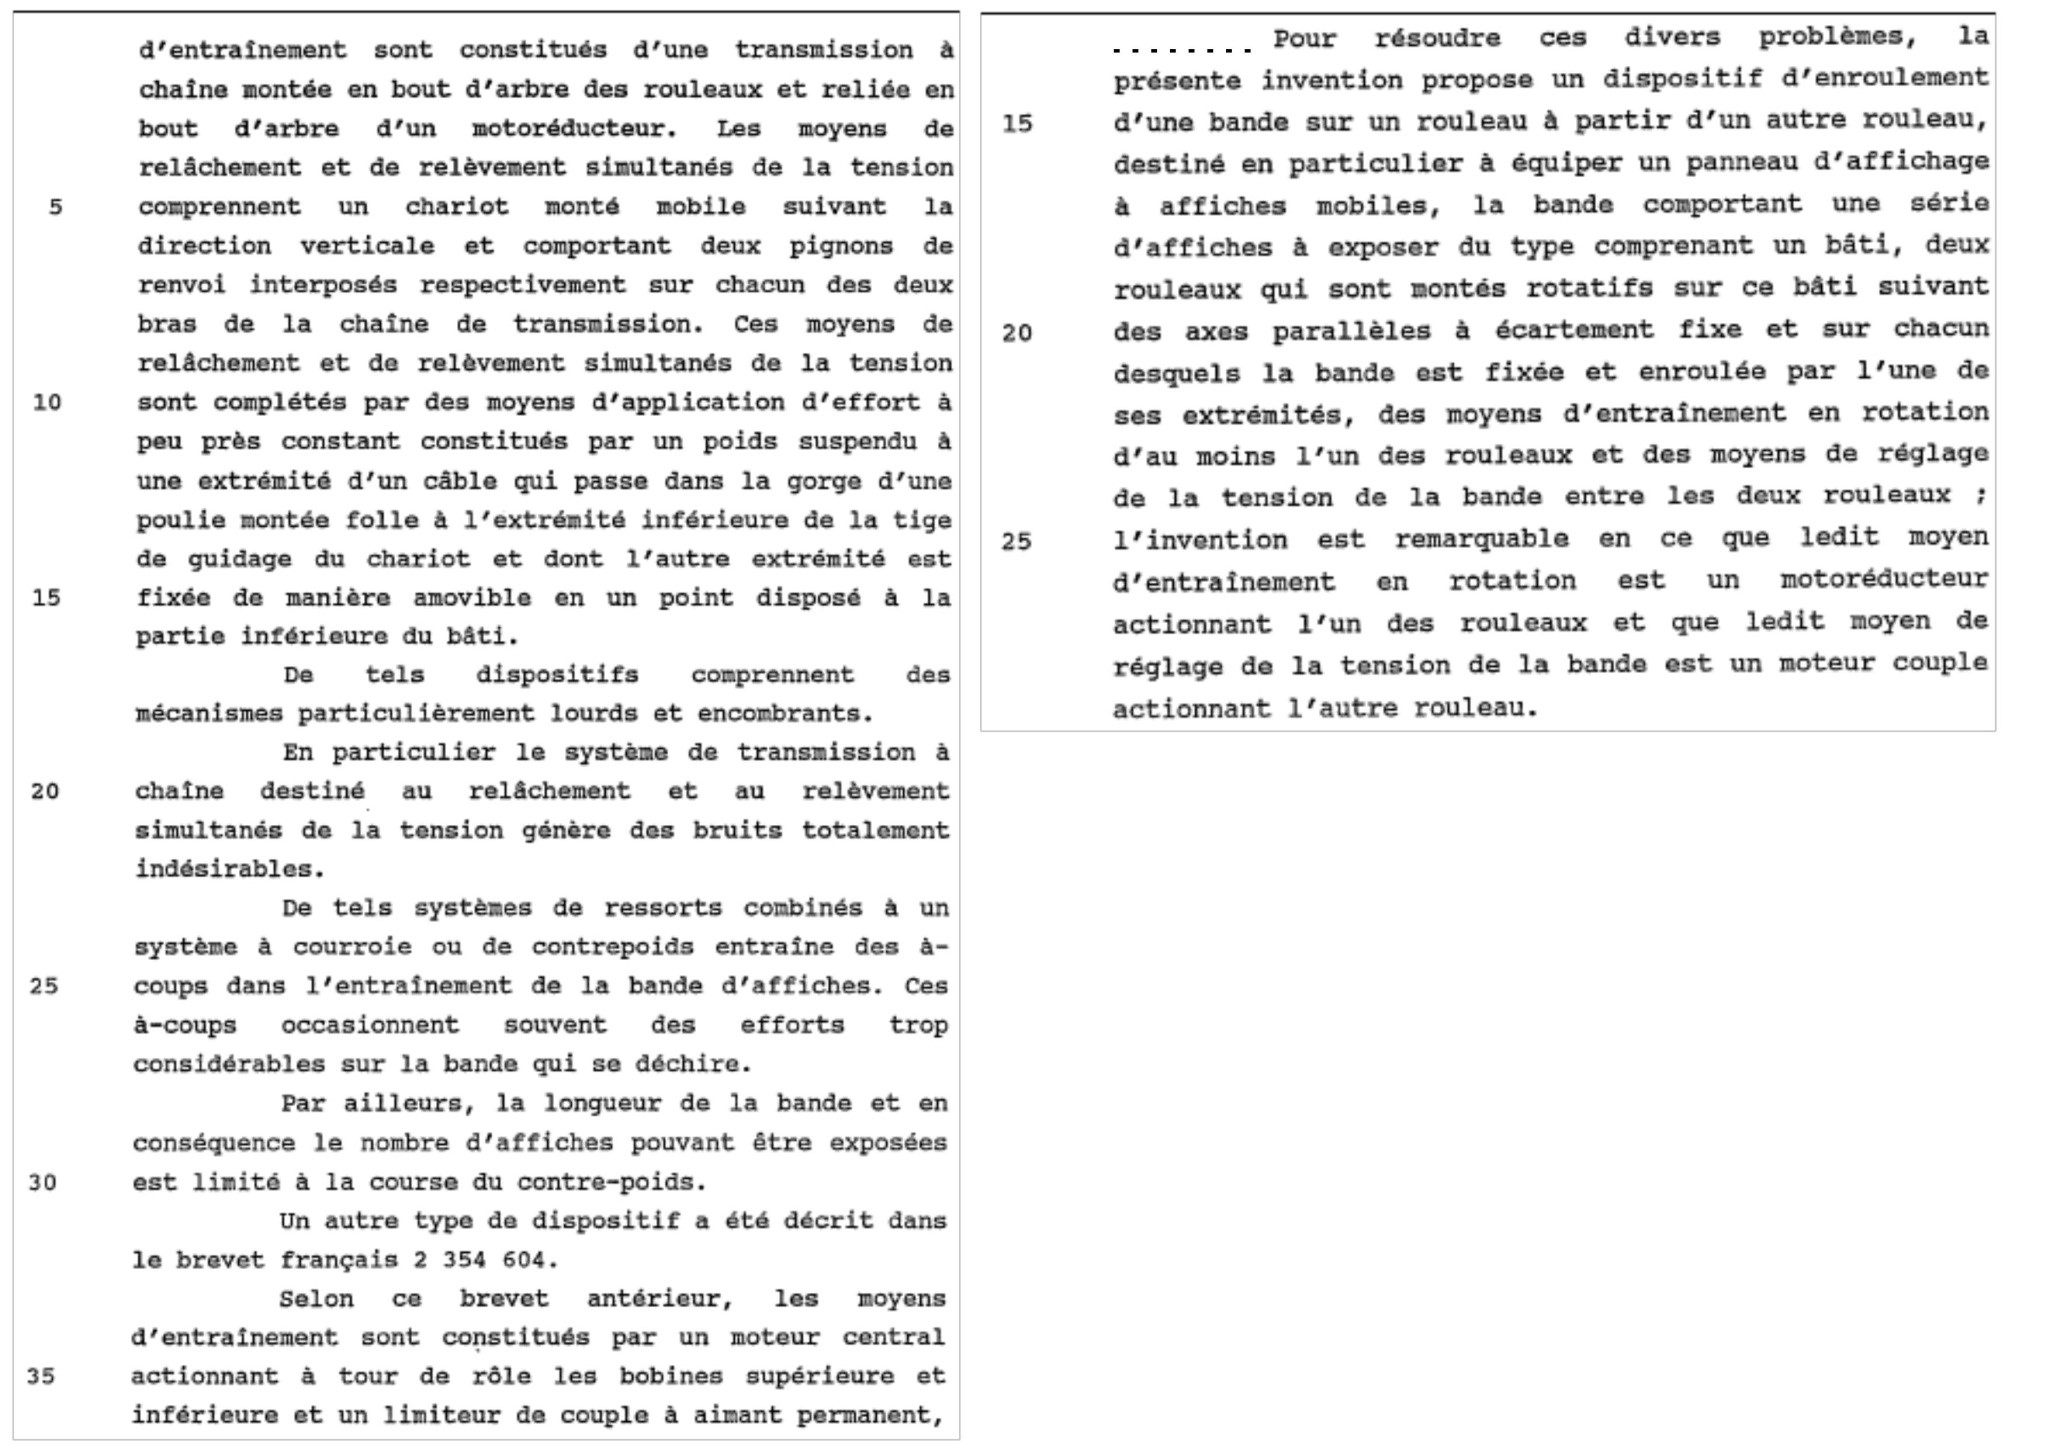
\includegraphics[width=0.9\linewidth]{img/annexe4_2}
\end{center}

\newpage

\textbf{Annexe 5}

\begin{center}
 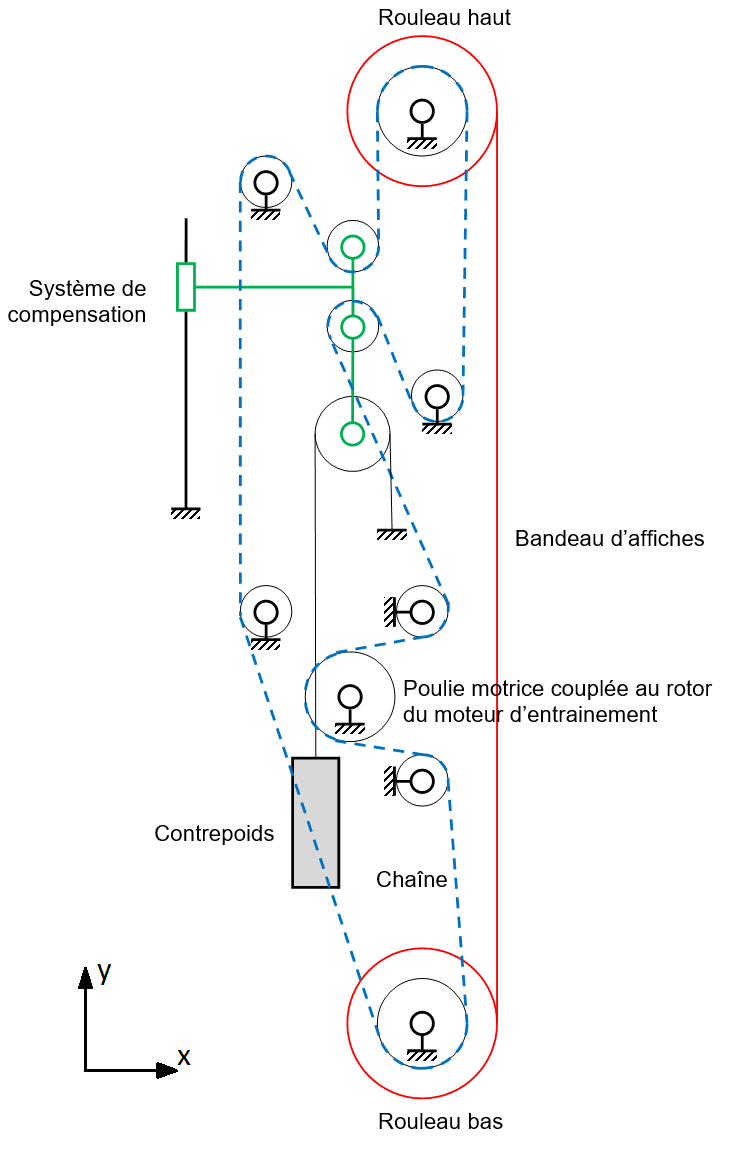
\includegraphics[width=0.8\linewidth]{img/annexe5}
\end{center}

\newpage

\textbf{Annexe 6}

\begin{center}
 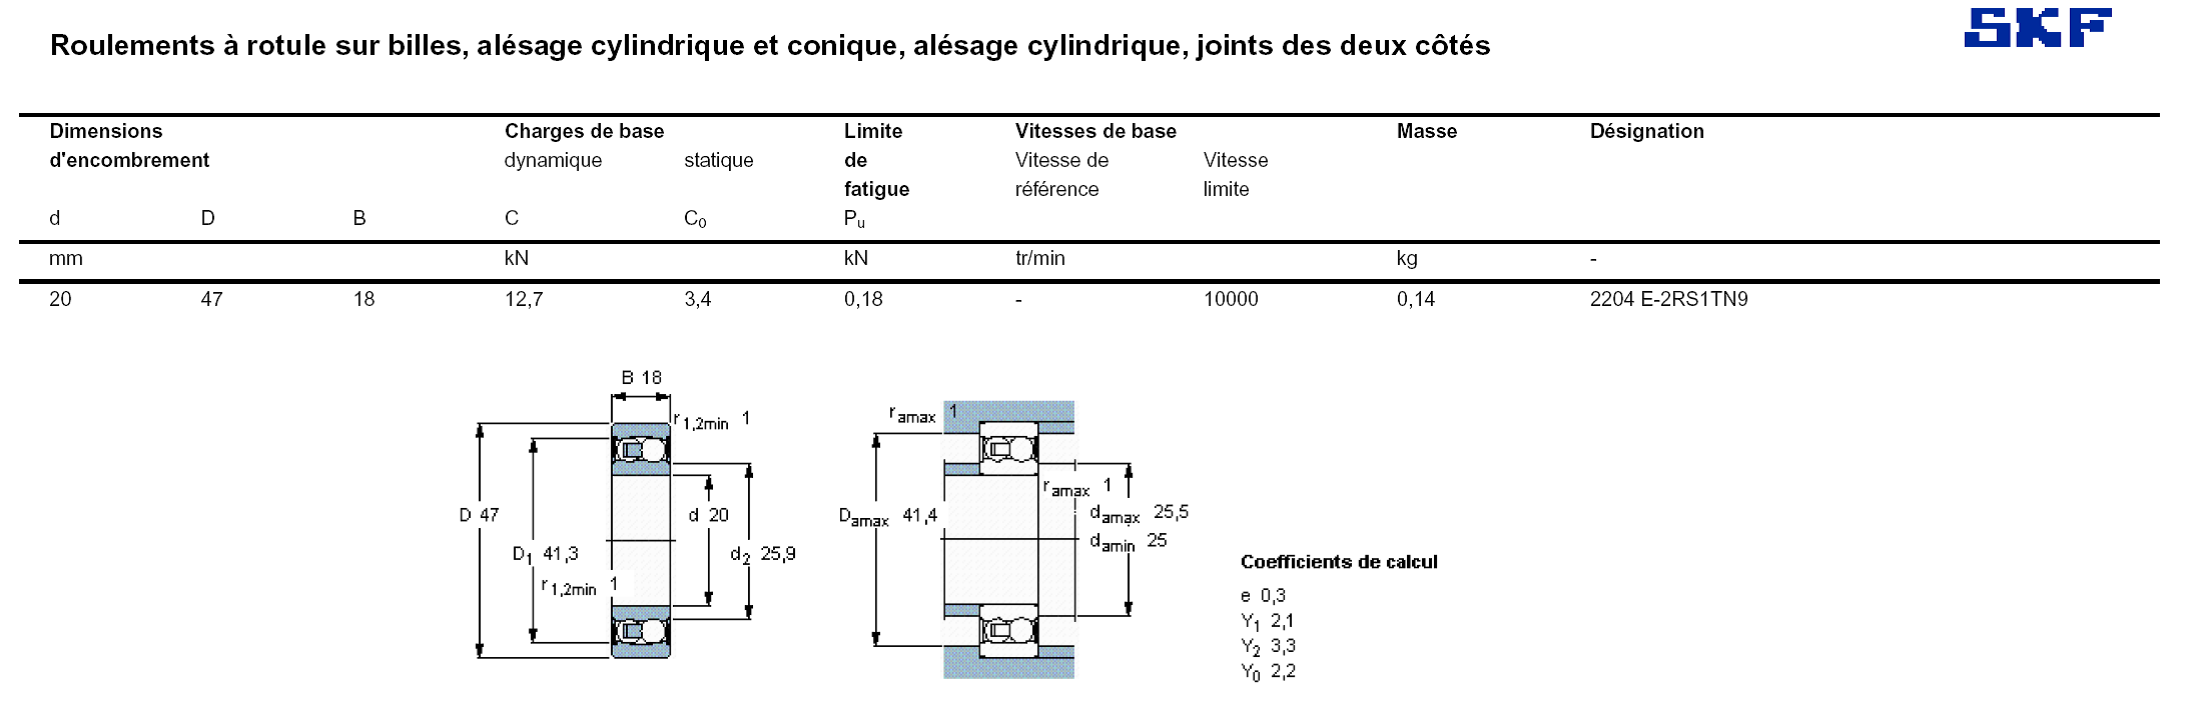
\includegraphics[width=0.9\linewidth]{img/annexe6_1}

~\

 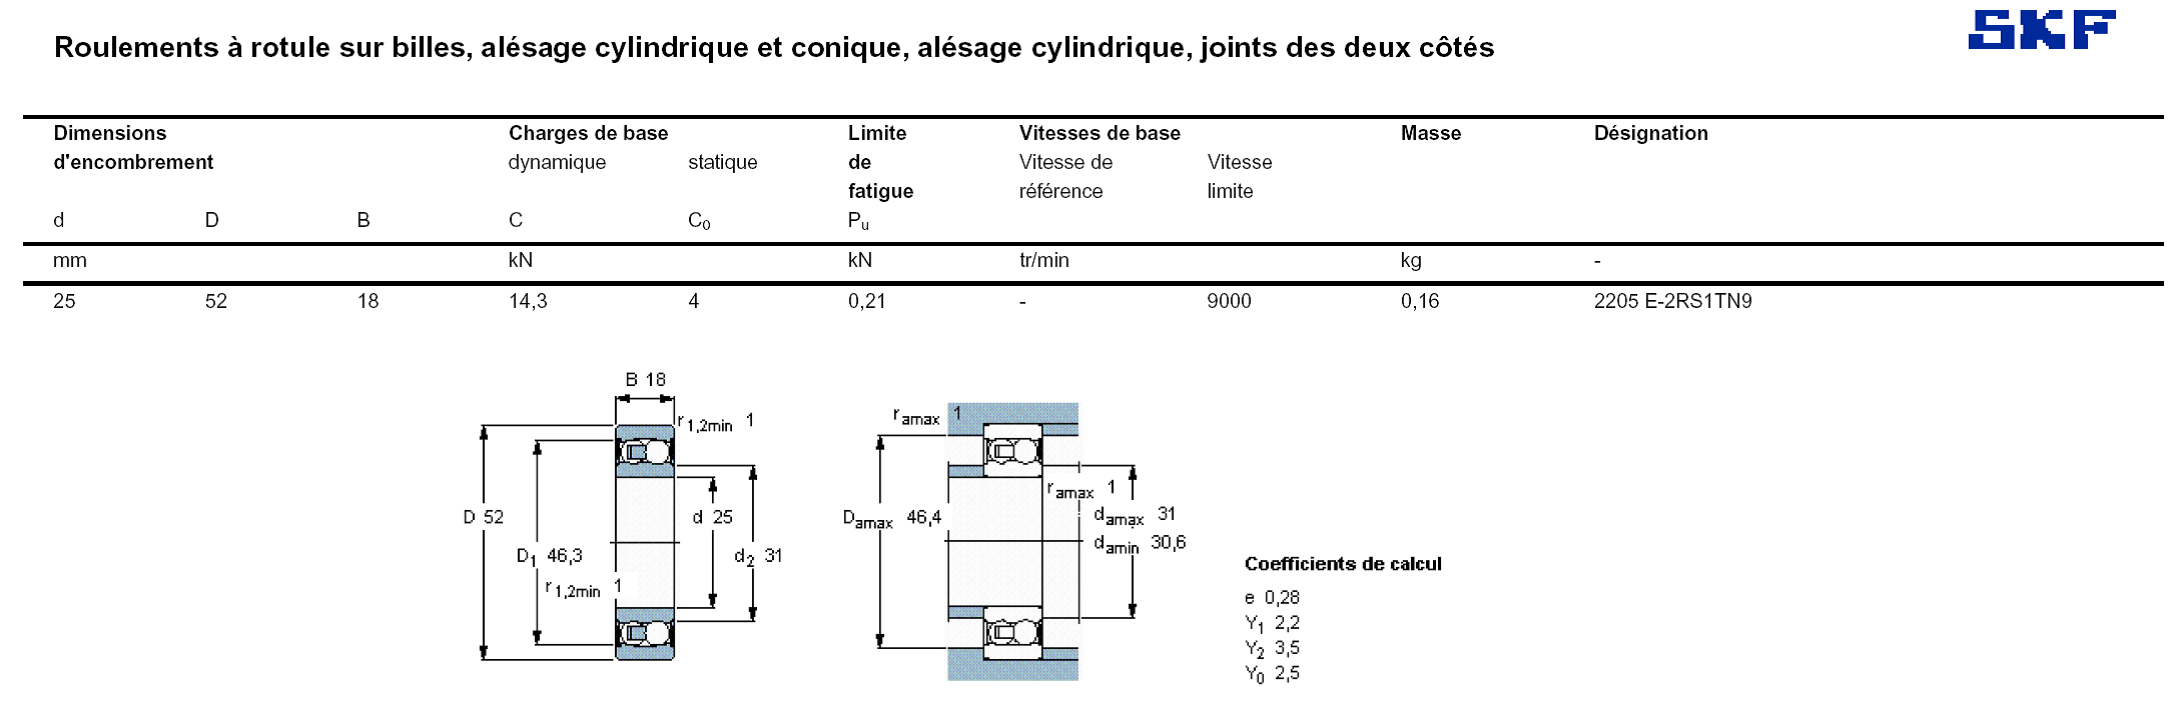
\includegraphics[width=0.9\linewidth]{img/annexe6_2}
\end{center}

\newpage

Document réponse

\begin{itemize}
 \item Nom=..............................
 \item Prénom=...........................
\end{itemize}

\begin{center}
 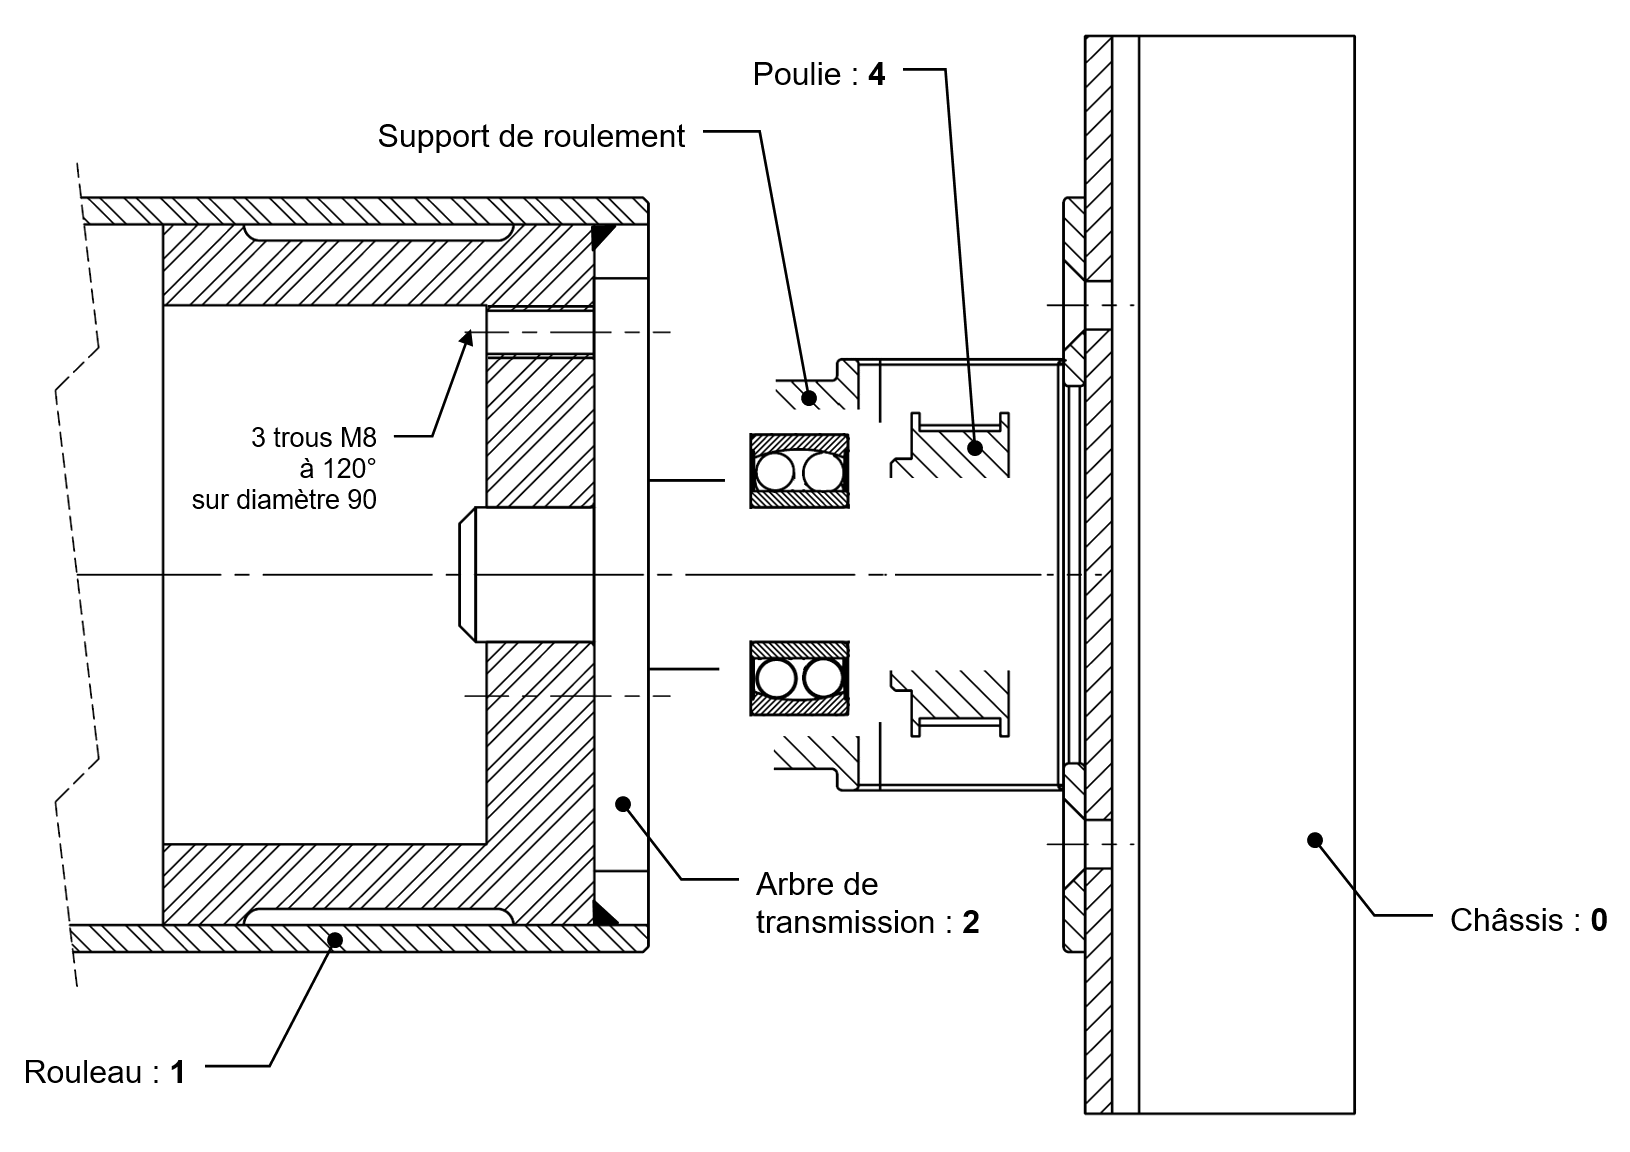
\includegraphics[angle=-90,width=0.9\linewidth]{img/DR2}
\end{center}

\ifdef{\public}{\end{document}}{}

\newpage
\cleardoublepage

\pagestyle{correction}

\setcounter{equation}{0}

\section{Correction}

\cor{$M_{roul}=\pi\cdot L\cdot\rho_{roul}\cdot\left(\frac{d_2^2}{4}-\frac{d_1^2}{4}\right)=3,14\cdot 3,2\cdot2700\cdot\left(\frac{0,0196}{4}-\frac{0,0166}{4}\right)\simeq3\cdot 3\cdot3\cdot\left(4,9-4,15\right)\simeq 20,25kg$}

\cor{$M_{b}=\pi\cdot L\cdot\rho_{b}\cdot\left(\frac{d_3^2}{4}-\frac{d_2^2}{4}\right)$}

\cor{$\left\{T_A\right\}=\left\{\begin{array}{cc}
X_A & 0 \\ Y_A & 0 \\ Z_A & 0 \end{array}\right\}_A=\left\{\begin{array}{cc}
X_A & 0 \\ Y_A & L.Z_A \\ Z_A & -L.Y_A \end{array}\right\}_B$

$\left\{T_A\right\}=\left\{\begin{array}{cc}
0 & 0 \\ Y_B & 0 \\ Z_B & 0 \end{array}\right\}_B$

$\left\{T_P\right\}=\left\{\begin{array}{cc}
0 & 0 \\ -P_{roul}-P_m & 0 \\ 0 & 0 \end{array}\right\}_B=\left\{\begin{array}{cc}
0 & 0 \\ -P_{roul}-P_m & 0 \\ 0 & \frac{L}{2}.(P_{roul}+P_m) \end{array}\right\}_B$

Donc, $X_A=0$, $Y_A=Y_B=\frac{P_{roul}+P_m}{2}$, $Z_A=Z_B=0$.}

\cor{Efforts radiaux: $F_r=\sqrt{Y_A^2+Z_A^2}=Y_A=\frac{P_{roul}+P_m}{2}$}

\cor{$R(t)=R_i+\frac{\theta(t)}{2.\pi}.e$, donc par dérivation $\frac{dR(t)}{dt}=\frac{d\theta(t)}{dt}.\frac{e}{2.\pi}=\Omega(t).\frac{e}{2.\pi}=\frac{V_0}{R(t)}.\frac{e}{2.\pi}$}

\cor{$R(0)=R_i$, $R(t).dR(t)=V_0.\frac{e}{2.\pi}.dt$, donc $\int_0^t R(t).dR(t)=\int_0^t V_0.\frac{e}{2.\pi}.dt$

$R^2(t)-R_i^2=V_0.\frac{e}{2.\pi}.t$, donc $R(t)=\sqrt{R_i^2+V_0.\frac{e}{\pi}.t}$}

\cor{$R(T_f)=\sqrt{70^2+10^3.0,2.\frac{14}{\pi}}\simeq76mm$.}

\cor{$\Omega_{min}=\frac{V_0}{R_f}\frac{1000}{76}\simeq 13rad.s^{-1}$ et $\Omega_{max}=\frac{V_0}{R_i}\frac{100}{7}\simeq 14,3rad.s^{-1}$}

\cor{$\frac{\Omega_{max}-\Omega_{min}}{\Omega_{max}}=\frac{1,3}{14,3}\simeq9\%$}

\cor{$d=(2.T_a-1).V_0$ donc $T_a=\frac{1}{2}.(\frac{d}{V_0}+1)=1,65s$}

\cor{$T_p=T_a-1=0,65s$}

\cor{Sens horaire}

\cor{C'est le contre-poids avec le système de compensation.}

\cor{Question ouverte mais quelques éléments de réponse:
\begin{itemize}
 \item Système lourd (contre-poids),
 \item Bruits,
 \item A-coups,
 \item Longueur de bande limitée.
\end{itemize}}

\cor{$V_0=k_r.K_{pc}.\Omega_m.R$}

\cor{$\gamma=\frac{dV_0}{dt}=k_r.K_{pc}.\dot{\Omega}_m.R$}

\cor{\begin{itemize}
\item $E(p)=k_e.\Omega_m(p)$,
\item $V_a(p)=R_a.I(p)+E(p)$,
\item $C_m(p)=k_c.I(p)$,
\item $J_{mc}.p.\Omega_m(p)=C_m(p)-C_r(p)$
\end{itemize}}

\cor{$A1(p)=\frac{1}{R_a}$, $A2(p)=k_c=k_e=k$, $A3(p)=\frac{1}{J_{mc}.p}$}

\cor{$C_m=A1.A2.(V_a-E)$, $V_a=H.(V_{10}-V_{lm})=H.(V_{10}-H_i.I)=H.(V_{10}-H_i.\frac{C_m}{A2})$, $E=A2.A3.(C_m-C_r)$, donc \\
$C_m(p)=\frac{A1.A2.H}{1+A1.H.H_i+A1.A2^2.A3}.V_{10}(p)+\frac{A1.A2^2.A3}{1+A1.H.H_i+A1.A2^2.A3}.C_r(p)$
}

\cor{$\Omega_m=A3.(C_m-C_r)$, $C_r=\lambda.(\Omega_m-\Omega_s)=\lambda.(A3.(C_m-C_r)-\Omega_s)$\\
donc

$C_m=\frac{A1.A2.H}{1+A1.H.H_i+A1.A2^2.A3}.V_{10}+\frac{A1.A2^2.A3}{1+A1.H.H_i+A1.A2^2.A3}.\left(\frac{\lambda.A3}{1+\lambda.A3}.C_m-\frac{\lambda}{1+\lambda.A3}.\Omega_s\right)$

donc

$C_m=\frac{A1.A2.H.(1+\lambda.A3)}{1+\lambda.A3+A1.H.H_i+\lambda.A1.A3.H.H_i+A1.A2^2.A3}.V_{10}+\frac{A1.A2^2.A3.\lambda}{1+\lambda.A3+A1.H.H_i+\lambda.A1.A3.H.H_i+A1.A2^2.A3}.\Omega_s$
}

\newpage

\cor{\begin{center}
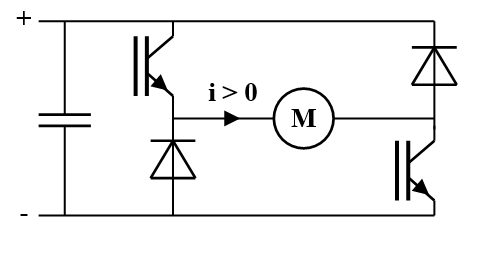
\includegraphics[width=0.5\linewidth]{img/schem_elec_cor}
\end{center}}

\cor{Filtre passe bas}

\cor{$V_A=\frac{\frac{V_{im}}{R}+\frac{V_{is}}{10.R}}{\frac{1}{R}+\frac{1}{10.R}+j.C.\omega}=\frac{10.V_{im}+V_{is}}{11+j.10.R.C.\omega}$}

\cor{$V_{is}=V_A.\frac{\frac{1}{j.\frac{C}{10}.\omega}}{10.R+\frac{1}{j.\frac{C}{10}.\omega}}=V_A.\frac{1}{1+j.R.C.\omega}$, ainsi 

$V_{is}=\frac{10.V_{im}+V_{is}}{(11+j.10.R.C.\omega).(1+j.R.C.\omega)}$

Donc

$\frac{V_{is}}{V_{im}}=\frac{1}{1+2,1.j.\frac{\omega}{\omega_0}+\left(\frac{\omega}{\omega_0}\right)^2}$, donc $\alpha=2,1$.}

\cor{C'est un filtre passe bas d'ordre 2, ainsi, la pente après la cassure est de -40dN/dec, il faut donc 1 décade pour une atténuation de 40dB, soit, $\omega_i=10.\omega_0$, donc $\omega_0=\frac{\omega_i}{10}=\frac{\frac{2.\pi}{0,5.10^{-3}}}{10}\simeq 1256rad.s^{-1}$}

\cor{$C=\frac{1}{R.\omega_0}=\frac{1}{10^4.1256}=79\eta F$}

\cor{$J_{mc}.\frac{d\Omega_m(t)}{dt}=\lambda.\left(\Omega_{s1}-\Omega_m\right)-\lambda.\left(\Omega_m-\Omega_{s2}\right)=\lambda.\left(\Omega_{s1}+\Omega_{s2}\right)-2.\lambda.\Omega_m$

En régime permanent, $\frac{d\Omega_m(t)}{dt}\rightarrow 0$, donc $\Omega_m\rightarrow \frac{\Omega_{s1}+\Omega_{s2}}{2}$.}

\cor{$\Delta\Omega_s=\Omega_{s1}-\Omega_{s2}=\Omega_{s1}-\left(2.\Omega_{m}-\Omega_{s1}\right)=2.\frac{C_m}{\lambda}=2.\frac{0,3}{0,05}=12rad.s^{-1}$

$\Delta_f=\frac{\Delta \Omega_s}{\pi}=\frac{12}{\pi}\simeq 3,8Hz$.}

\cor{$h=3+3-(6(2-1)-1)=1$}

\cor{Il faut prévoir un réglage, ce qui est fait grâce à la liaison pivot glissant et vis de pression entre 1 et 3.}

\cor{Ces roulements à deux rangées de billes permettent un fort rotulage ce qui est nécessaire à cette solution.}

\cor{La pression sur la courroie ne sera pas uniforme sur toute sa largeur ce qui peut provoquer une dégradation plus rapide.}

\cor{\begin{center}
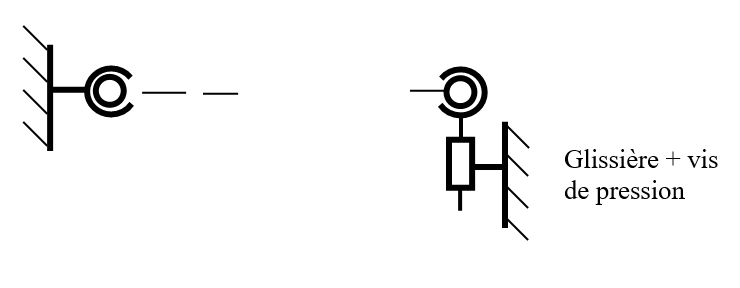
\includegraphics[width=0.7\linewidth]{img/solution_reglage}
\end{center}}

\cor{$h=4+4-(6(2-1)-2)=4$, il faudrait pour que cela s'assemble que les deux portées de roulement soient coaxiales.}

\cor{\begin{center}
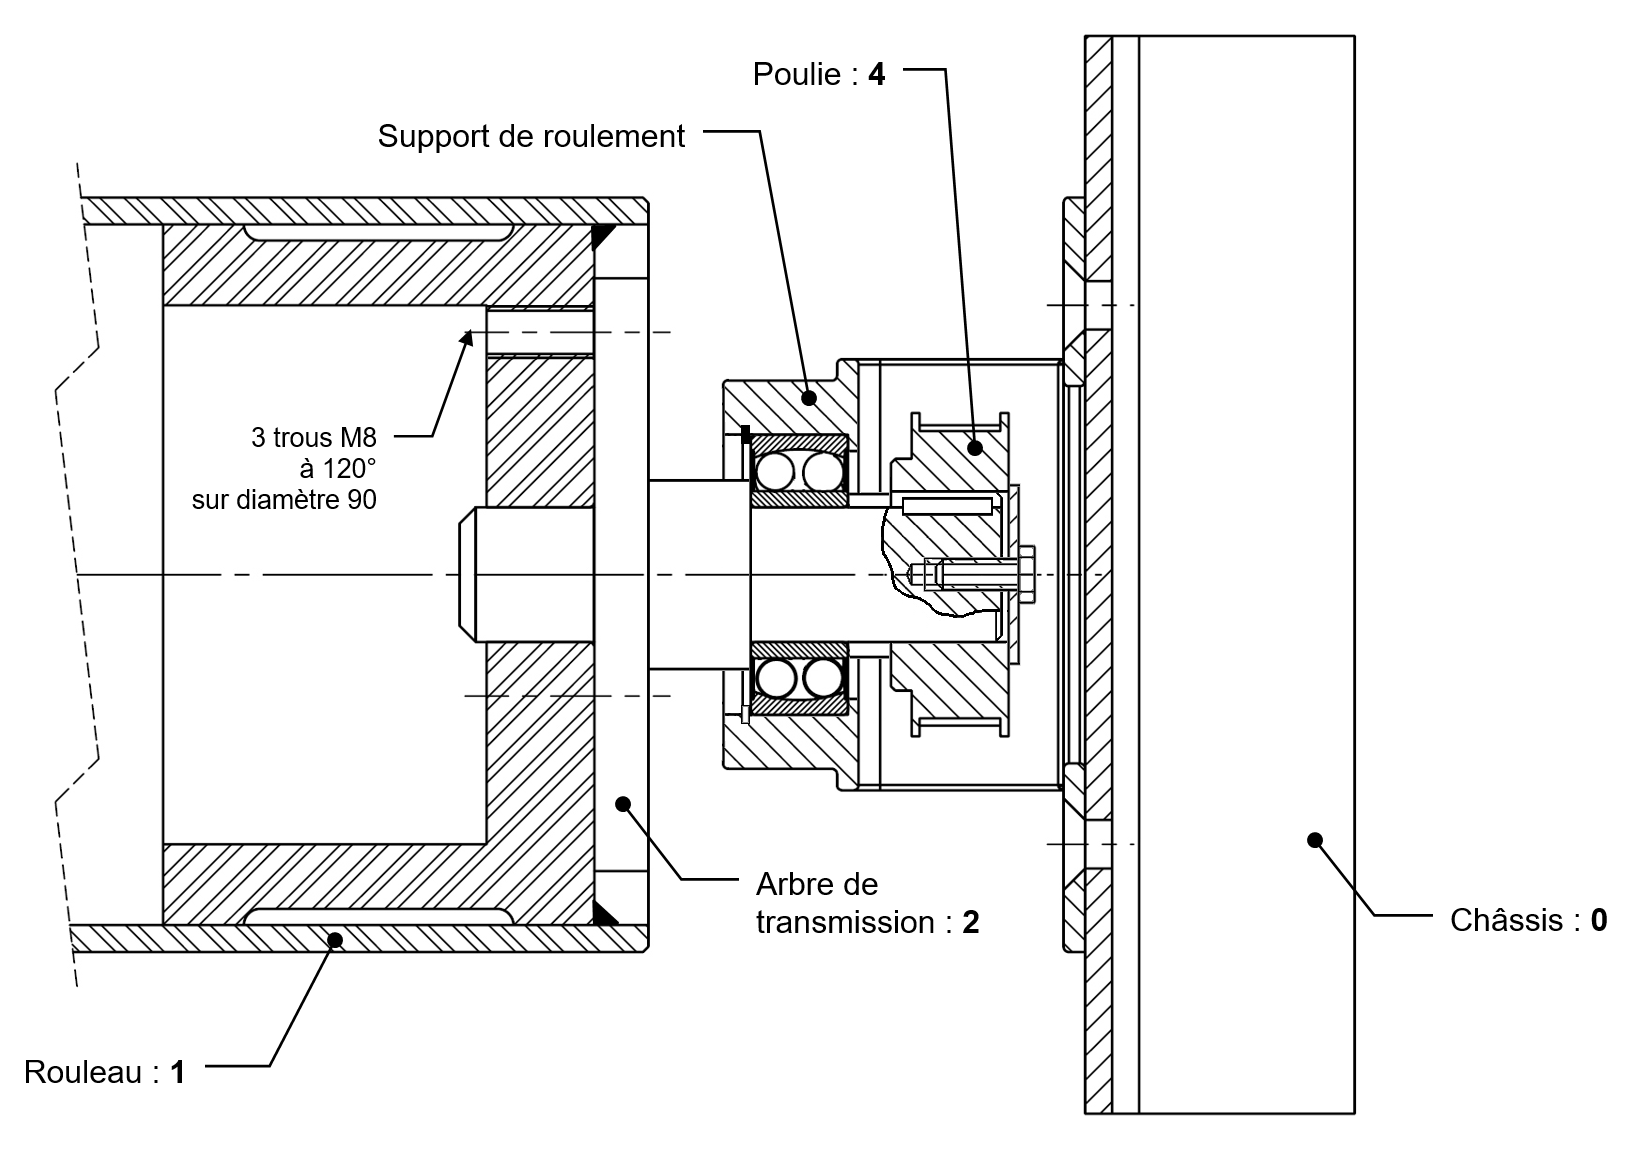
\includegraphics[width=0.7\linewidth]{img/DR2_cor}
\end{center}}

\end{document}
